\chapter{numeri e funzioni}


\section{proposizioni e predicati}

Se, come diceva Galileo, la matematica è il linguaggio della scienza,
è importante che la matematica sia essa stessa espressa in un linguaggio
che risulti essere il più possibile oggettivo e non ambiguo.
La \emph{logica} è la disciplina matematica che si occupa
dello studio e della formalizzazione del linguaggio matematico.
In questo capitolo riassumiamo in maniera breve ed intuitiva
alcuni concetti che probabilmente sono noti e contemporaneamente
fissiamo le notazioni che verranno utilizzate nel seguito.
Per eventuali approfondimenti rimandiamo a \cite{appunti_logica}.

Una \myemph{proposizione}
è una frase (formalmente diremmo \emph{formula})
che assume un valore di verità ben
definito: vero oppure falso.
Un esempio di proposizione (falsa) è ``2+2=5''.

E' possibile combinare più proposizioni mediante
gli operatori logici. Se $P$ e $Q$ sono proposizioni
si può costruire la proposizione $P \land Q$
chiamata \myemph[congiunzione]{congiunzione logica}.
Tale proposizione
si può leggere ``$P$ e $Q$'' ed è una proposizione
che risulta essere vera solamente nel caso in cui sia
$P$ che $Q$ siano vere.
La \myemph[disgiunzione]{disgiunzione logica} denotata
con $P \lor Q$
si può leggere ``$P$ o $Q$'' ed è una proposizione che
è vera se almeno una tra $P$ e $Q$ è vera.
La \myemph[negazione]{negazione logica} denotata con $\lnot P$ è una
proposizione che si può leggere ``non $P$'' che
è vera quando $P$ è falsa ed è falsa quando $P$ è vera.

Operatori logici molto utilizzati sono le \myemph{implicazioni}.
La proposizione $P\Rightarrow Q$ si può leggere ``$P$ implica $Q$''
e significa che $Q$ è vera se $P$ è vera. Non si confonda
il valore di verità di $P\Rightarrow Q$ con il valore di verità
di $Q$. Se $P$ è vera allora $P\Rightarrow Q$ è vera o falsa
a seconda che $Q$ sia vera o falsa. Ma se $P$ è falsa allora
l'implicazione $P\Rightarrow Q$ è vera indipendentemente dal
valore di $Q$. In effetti $P\Rightarrow Q$ è equivalente a
$Q \lor \lnot P$ perché per la verità di $P\Rightarrow Q$
basta che $Q$ sia vera (quando $P$ è vera) oppure che $P$ sia falsa.

La freccia inversa $P\Leftarrow Q$ si può utilizzare per
invertire l'implicazione: è equivalente a $Q \Rightarrow P$.
Se valgono entrambe le implicazioni
$(P \Leftarrow Q) \land (P\Rightarrow Q)$
è facile convincersi che $P$ e $Q$ devono avere lo stesso
valore di verità: diremo quindi che sono equivalenti e
scriveremo $P \Leftrightarrow Q$.

Nella tabella~\ref{tab:verita_operatori_logici} sono riportati
tutti i valori di verità che si possono ottenere combinando
tra loro due proposizioni. Nella tabella~\ref{tab:operatori_logici}
sono riportate alcune proprietà di tali operatori: queste
proprietà possono essere capite interpretando il loro significato
ma possono anche essere dedotte meccanicamente tramite la tabella
di verità delle operazioni.

\begin{table}
\begin{center}
  \begin{tabular}{cc|cccccc}
    $P$ & $Q$ & $\neg P$ & $P\land Q$ & $P\lor Q$ & $P\Rightarrow Q$ &
    $P\Leftarrow Q$ & $P\Leftrightarrow Q$ \\\hline
    \texttt{V} & \texttt{V} & \texttt{F} & \texttt{V} & \texttt{V} & \texttt{V} & \texttt{V} & \texttt{V} \\
    \texttt{V} & \texttt{F} & \texttt{F} & \texttt{F} & \texttt{V} & \texttt{F} & \texttt{V} & \texttt{F} \\
    \texttt{F} & \texttt{V} & \texttt{V} & \texttt{F} & \texttt{V} & \texttt{V} & \texttt{F} & \texttt{F} \\
    \texttt{F} & \texttt{F} & \texttt{V} & \texttt{F} & \texttt{F} & \texttt{V} & \texttt{V} & \texttt{V} \\
    \end{tabular}
\end{center}
\caption{La tabella di verità degli operatori logici.}
\label{tab:verita_operatori_logici}
\end{table}

\begin{table}
\begin{tabular}{rcll}
                         $\neg \neg P$ & $\iff$ & $ P$                           & doppia negazione\\
                                    $P \land Q$ & $\iff$ & $ Q \land P$                   & simmetria\\
                                     $P \lor Q$ & $\iff$ & $ Q \lor P$                    & \\
                              $\neg (P\land Q)$ & $\iff$ & $ (\neg P) \lor (\neg Q)$      & formule di De Morgan\\
                               $\neg (P\lor Q)$ & $\iff$ & $ (\neg P) \land (\neg Q)$     & \\
                            $(P\land Q) \lor R$ & $\iff$ & $ (P\lor R) \land (Q \lor R)$  & proprietà distributiva\\
                            $(P\lor Q) \land R$ & $\iff$ & $ (P\land R) \lor (Q \land R)$ & \\
                            $(P \Rightarrow Q)$ & $\iff$ & $ (Q \Leftarrow P)$            & antisimmetria\\
                        $\neg (P\Rightarrow Q)$ & $\iff$ & $ P \land (\neg Q)$            & controesempio\\
                             $(P\Rightarrow Q)$ & $\iff$ & $ \lnot(P \land (\neg Q))$     & dimostrazione per assurdo\\
                             $(P\Rightarrow Q)$ & $\iff$ & $ (\neg Q\Rightarrow\neg P)$   & implicazione contropositiva
\end{tabular}
\caption{Alcune proprietà degli operatori logici.}
\label{tab:operatori_logici}
\end{table}

Un \myemph{predicato} è una proposizione che contiene
una o più variabili, il cui valore di verità, quindi,
può dipendere dal valore assegnato alle variabili.
Un esempio di predicato è $x+2=5$ che risulta essere vero se $x=3$
e falso altrimenti.

Se un predicato dipende da una o più variabili queste
si chiamano \myemph{variabili libere}. E' possibile
\emph{chiudere} una variabile libera mediante un quantificatore.
Il \myemph{quantificatore universale} denotato col simbolo
$\forall$ serve ad affermare che il predicato è vero
per ogni possibile valore della variabile quantificata.
Ad esempio la proposizione $\forall x\colon x+2=5$ significa:
``per ogni $x$ si ha $x+2=5$'' ed è una proposizione falsa.
Il quantificatore $\forall x$ rende \emph{muta} la variabile
$x$ del predicato $x+2=5$ nel senso che la proposizione
non dipende più dal valore di quella variabile, che non è
più una variabile libera.

Il \myemph{quantificatore esistenziale} denotato col simbolo
$\exists$ serve ad affermare che il predicato è vero per
almeno un valore della variabile quantificata.
Ad esempio la proposizione $\exists x\colon x+2=5$ significa:
``esiste almeno un $x$ per cui risulta $x+2=5$''.
Quello che si ottiene è una proposizione in cui la variabile
$x$ è muta. In questo caso la proposizione è vera in quanto
per $x=3$ il predicato è vero.

Un predicato può dipendere da più variabili ed è quindi
possibile inserire più quantificatori. In tal caso l'ordine
dei quantificatori può essere rilevante.
Delle seguenti proposizioni la prima è vera, la seconda
invece è falsa:
\begin{gather*}
\forall x\colon \exists y\colon x+2=y \\
\exists y\colon \forall x\colon x+2=y.
\end{gather*}

\begin{table}
\begin{center}
\begin{tabular}{lcl}
$\lnot \forall x \colon P(x)$ & $\iff$ & $\exists x \colon \lnot P(x)$\\
$\lnot \exists x \colon P(x)$ & $\iff$ & $\forall x \colon \lnot P(x)$\\
$\forall x \colon P(x)$ & $\Longrightarrow$ & $\exists x \colon P(x)$
\end{tabular}
\end{center}
\caption{Alcune proprietà dei quantificatori logici.}
\label{tab:proprieta_quantificatori}
\end{table}

Alcune proprietà dei quantificatori logici sono riportate
nella tabella~\ref{tab:proprieta_quantificatori}.


\section{teoria degli insiemi}
Nei paragrafi precedenti abbiamo visto che i predicati possono essere
combinati tra loro e quantificati.
Ma quali sono i predicati elementari che possiamo considerare?
La teoria degli insiemi ci fornisce la formalizzazione del concetto
di \emph{appartenenza}: il predicato di base (l'unico che ci servirà) è
un predicato della forma $x \in A$ che significa ``l'oggetto $x$ è un elemento
dell'insieme $A$''.
La teoria degli insiemi non spiega (né tantomento definisce)
cosa siano gli oggetti e cosa siano gli insiemi perché questi sono concetti
primitivi (come lo sono i \emph{punti} e le \emph{rette} per la geometria euclidea).
La teoria degli insiemi ci fornisce, semplicemente, le regole formali che
possono essere utilizzate per trattare i predicati della forma $x\in A$.
Ad esempio un \emph{assioma} della teoria degli insiemi è il seguente:
\[
  \exists A \colon \lnot \exists x\colon x \in A
\]
che significa: ``esiste un insieme $A$ che non contiene alcun elemento $x$''
ovvero stiamo dicendo che esiste l'\myemph{insieme vuoto} che normalmente viene
denotato con il simbolo $\emptyset$.
Altri opportuni assiomi della teoria degli insiemi garantiscono l'esistenza
dell'unione $A\cup B$, intersezione $A\cap B$ e differenza $A\setminus B$
di due insiemi qualunque $A$ e $B$. Tali operazioni
tra insiemi possono essere ricondotte alla relazione di appartenenza
e possono quindi essere definite come segue:
\begin{align*}
    x \in A \cup B &\iff (x\in A) \lor (x\in B)\\
    x \in A \cap B &\iff (x\in A) \land (x\in B)\\
    x \in A \setminus B &\iff (x\in A) \land \lnot (x \in B).
\end{align*}
La negazione dell'appartenenza $\lnot (x \in A)$ viene usualmente
abbreviata con $x \not \in A$.

Sempre utilizzando la semplice relazione di appartenenza possiamo definire
le relazioni di inclusione e uguaglianza tra insiemi:
$A \subset B$ si legge ``$A$ è un sottoinsieme di $B$''
e $A=B$ si legge ``$A$ è uguale a $B$''. Queste relazioni sono
definite dalle seguenti proprietà:
\begin{align*}
  A \subset B &\iff \forall x\colon (x\in A \implies x\in B)\\
  A = B &\iff \forall x\colon (x\in A \iff x \in B).
\end{align*}
Ovviamente la relazione $A \subset B$ può essere invertita: scriveremo
$A\supset B$ (che si può leggere: ``$A$ è un soprainsieme di $B$'')
per indicare $B \subset A$. Scriveremo anche $A \neq B$ per indicare
la relazione opposta dell'uguaglianza ovvero: $\lnot(A=B)$.

Risulta molto utile la possibilità di costruire insiemi di insiemi.
Per questo motivo la teoria degli insiemi usualmente non fa distinzione
tra oggetti e insiemi di oggetti. Nella relazione primitiva $x\in A$ anche
$x$ può essere un insieme. Possiamo allora immaginare che ogni oggetto del
nostro universo sia un insieme. In questo modo la relazione di uguaglianza $A=B$
che abbiamo definito sopra risulta ben definita per ogni coppia di oggetti
(o insiemi, che è lo stesso) $A$ e $B$.

Visto che gli elementi di un insieme $\mathcal A$ sono a loro volta insiemi,
è possibile considerare l'unione $\bigcup \mathcal A$
e l'intersezione $\bigcap \mathcal A$ di tutti gli elementi
di $\mathcal A$.
Questo estende il concetto di unione e intersezione anche a famiglie
eventualmente infinite:
\begin{align*}
  x \in \bigcup \mathcal A & \iff \exists A \in \mathcal A \colon x\in A, \\
  x \in \bigcap \mathcal A & \iff \forall A \in \mathcal A \colon x\in A.
\end{align*}

Un altro assioma della teoria degli insiemi garantisce che per ogni
$x$ esiste un insieme il cui unico elemento è $x$. Tale insieme
si chiama \emph{singoletto} e si denota con $\ENCLOSE{x}$. La proprietà
che definisce il singoletto è la seguente:
\[
  y \in \ENCLOSE{x} \iff y=x.
\]
Facendo l'unione di singoletti possiamo definire (per elencazione) insiemi che contengono
un numero finito di oggetti:
\begin{align*}
  \ENCLOSE{a,b} &= \ENCLOSE{a} \cup \ENCLOSE{b} \\
  \ENCLOSE{a, b, c} &= \ENCLOSE{a,b} \cup \ENCLOSE{c}\\
  \ENCLOSE{a, b, c, d} &= \ENCLOSE{a,b,c} \cup \ENCLOSE{d}\\
  &\quad\vdots
\end{align*}

Si faccia però attenzione: l'insieme $\ENCLOSE{a,b}$ contiene due elementi
solamente se $a\neq b$, infatti se $a=b$ si potrà facilmente verificare
che
\begin{equation}\label{eq:4775523}
\ENCLOSE{a,a} = \ENCLOSE{a}.
\end{equation}

\begin{exercise}
  Verificare \eqref{eq:4775523} utilizzando le definizioni formali date in precedenza.
\end{exercise}
\begin{proof}[Svolgimento.]
Utilizzando le definizioni di unione, di singoletto e di disgiunzione logica
si ha l'equivalenza dei seguenti
predicati:
\begin{gather*}
  x \in \ENCLOSE{a,a}  \\
  x \in \ENCLOSE{a} \cup \ENCLOSE{a}\\
  (x \in \ENCLOSE{a}) \lor (x \in \ENCLOSE{a})\\
  (x = a) \lor (x = a) \\
  x = a \\
  x \in \ENCLOSE{a}
\end{gather*}
e dunque $\ENCLOSE{a,a}=\ENCLOSE{a}$ per la definizione di uguaglianza tra insiemi.
\end{proof}

Se $P(x)$ è un predicato in una sola variabile $x$ vorremmo poter
definire l'insieme, denotato con $\ENCLOSE{x\colon P(x)}$
di tutti gli oggetti $x$ che rendono vero il predicato $P(x)$:
\[
  a \in \ENCLOSE{x\colon P(x)} \iff P(a).
\]
Sorprendentemente se inseriamo questo assioma nella teoria degli insiemi
si giunge ad un paradosso (paradosso di Russell, si veda \cite{appunti_logica})
e si ottiene quindi una teoria incoerente
(cioè una teoria in cui tutte le proposizioni sono vere). Per evitare
l'incoerenza è necessario limitare l'assioma (chiamato \emph{assioma di specificazione})
alla costruzione di sottoinsiemi di insiemi già costruiti.
Se $B$ è un insieme e $P(x)$ è un predicato possiamo considerare
l'insieme $\ENCLOSE{x\in B\colon P(x)}$ che è il sottoinsieme di
$B$ formato da tutti gli elementi di $B$
che soddisfano il predicato:
\[
  a \in \ENCLOSE{x\in B\colon P(x)} \iff (a \in B \land P(a)).
\]

Per completare la teoria degli insiemi introduciamo anche il concetto di
\myemph{insieme delle parti}. Un apposito assioma garantisce
che dato un qualunque insieme $A$ esiste l'insieme $\P(A)$ delle parti di $A$
che è l'insieme di tutti i sottoinsiemi di $A$:
\begin{equation}\label{eq:insieme_delle_parti}
  x \in P(A) \iff x \subset A.
\end{equation}

\begin{comment}
\section{numeri naturali}
%
La teoria degli insiemi prevede che ogni ``oggetto''
sia in effetti un insieme.
Possiamo ad esempio definire i numeri naturali partendo dall'insieme
vuoto e costruendo insiemi di insiemi, così:
\begin{align*}
  0 = \emptyset, \qquad
  1 = \ENCLOSE{0}, \qquad
  2 = \ENCLOSE{0,1}, \qquad
  3 = \ENCLOSE{0,1,2}, \qquad
  4 = \ENCLOSE{0,1,2,3}, \\
  5 = \ENCLOSE{0,1,2,3,4}, \qquad
  6 = \ENCLOSE{0,1,2,3,4,5}, \qquad
  7 = \ENCLOSE{0,1,2,3,4,5,6}, \\
  8 = \ENCLOSE{0,1,2,3,4,5,6,7}, \qquad
  9 = \ENCLOSE{0,1,2,3,4,5,6,7,8}.
\end{align*}
Risulta quindi che l'$n$-esimo numero naturale coincide
con l'insieme dei primi $n$ numeri naturali.
Ovviamente potremmo andare avanti: se $n$ è un numero naturale
il successivo non è altro che $n\cup \ENCLOSE{n}$.
\end{comment}

\section{relazioni e funzioni}

Grazie agli assiomi precedenti è possibile definire il prodotto cartesiano
di due insiemi: sarà questo un concetto molto importante nel seguito.
Innanzitutto dobbiamo definire il concetto di \myemph{coppia}: dati
$a,b$ definiamo la coppia $(a,b)$ con primo elemento $a$ e secondo elemento $b$
come un oggetto che ha questa proprietà:
\[
  (a, b) = (a', b') \iff (a=a') \land (b=b').
\]
Stiamo cioè richiedendo che una coppia viene identificata dai due
elementi che la compongono in cui, però, è importante anche l'ordine in
cui vengono elencati (a differenza dell'insieme $\ENCLOSE{a,b}$, in cui
l'ordine degli elementi è irrilevante).

Il \emph{prodotto cartesiano} $A\times B$ di due insiemi $A$ e $B$
è l'insieme di tutte le coppie il cui primo elemento sta in $A$ e
il secondo elemento sta in $B$:
\[
  (a, b) \in A \times B \iff (a\in A \land b\in B).
\]
Coppia e prodotto cartesiano possono essere definiti tramite gli
assiomi precedenti (si veda, al solito, \cite{appunti_logica})
ma non è veramente rilevante il modo in cui questo può essere fatto.

Se rappresentiamo gli elementi di $A$ come dei punti su una retta
orizzontale (asse delle $x$) e gli elementi di $B$ come dei punti
su una retta verticale (asse delle $y$) gli elementi di $A\times B$
possono essere rappresentati come i punti del piano che proiettati sull'asse
delle $x$ vanno in $A$ e proiettati sull'asse delle $y$ vanno in $B$.

\begin{figure}
  \hfill
  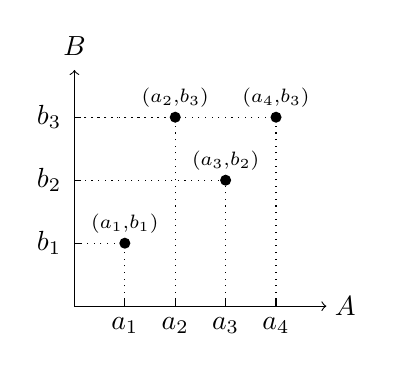
\begin{tikzpicture}[x=0.8cm]
  	\draw[->] (0,0) -- (4,0);
  	\draw[->] (0,0) -- (0,3);
  	\node at (4.3,0) {$A$};
  	\node at (0,3.3) {$B$};

      \draw (0.8,0) -- +(0,0.1) node [label=below:$a_1$]{};
      \draw (1.6,0) -- +(0,0.1) node [label=below:$a_2$]{};
      \draw (2.4,0) -- +(0,0.1) node [label=below:$a_3$]{};
      \draw (3.2,0) -- +(0,0.1) node [label=below:$a_4$]{};

      \draw (0,0.8) -- +(0.1,0) node [label=left:$b_1$]{};
      \draw (0,1.6) -- +(0.1,0) node [label=left:$b_2$]{};
      \draw (0,2.4) -- +(0.1,0) node [label=left:$b_3$]{};

  	\draw[dotted] (0.8,0) -- (0.8,0.8) -- (0,0.8);
  	\draw[dotted] (1.6,0) -- (1.6,2.4) -- (0,2.4);
  	\draw[dotted] (2.4,0) -- (2.4,1.6) -- (0,1.6);
  	\draw[dotted] (3.2,0) -- (3.2,2.4) -- (0,2.4);

  	\fill (0.8,0.8) circle (2pt) node[above] {$\scriptstyle (a_1,b_1)$};
  	\fill (1.6,2.4) circle (2pt) node[above] {$\scriptstyle (a_2,b_3)$};
  	\fill (2.4,1.6) circle (2pt) node[above] {$\scriptstyle (a_3,b_2)$};
  	\fill (3.2,2.4) circle (2pt) node[above] {$\scriptstyle (a_4,b_3)$};
  \end{tikzpicture}
%
  \hfill
%
  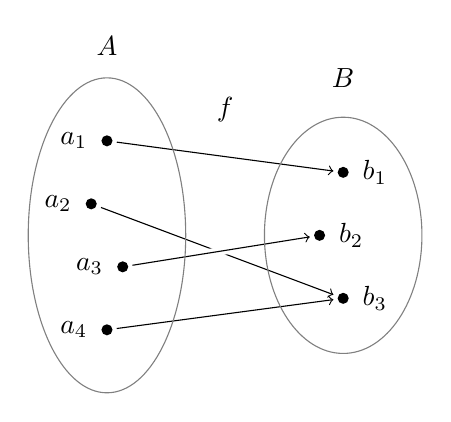
\begin{tikzpicture}[x=1cm,y=0.8cm]
  \fill (1,4) circle (2pt) node (a1) [label=left:$a_1$]{};
  \fill (0.8,3) circle (2pt) node (a2) [label=left:$a_2$]{};
  \fill (1.2,2) circle (2pt) node (a3) [label=left:$a_3$]{};
  \fill (1,1) circle (2pt) node (a4) [label=left:$a_4$]{};

  \fill (4,3.5) circle (2pt) node (b1) [label=right:$b_1$] {};
  \fill (3.7,2.5) circle (2pt) node (b2) [label=right:$b_2$] {};
  \fill (4,1.5) circle (2pt) node (b3) [label=right:$b_3$] {};

  \draw[->] (a1) edge (b1);
  \draw[->] (a2) edge (b3);
  \draw[line width=3pt,white] (a3) edge (b2);
  \draw[->] (a3) edge (b2);
  \draw[->] (a4) edge (b3);

  \draw[draw=gray](1,2.5) ellipse (1cm and 2cm);
  \draw[draw=gray](4,2.5) ellipse (1cm and 1.5cm);
  \node at (1,5.5) {$A$};
  \node at (4,5) {$B$};
  \node at (2.5,4.5) {$f$};
  \end{tikzpicture}
  \hfill
  \mbox{}
  \caption{La funzione $f\colon A\to B$,
  $f=\ENCLOSE{a_1\mapsto b_1,\ a_2 \mapsto b_3,\ a_3 \mapsto b_2,\ a_4 \mapsto b_3}$
  rappresentata tramite grafico e
  tramite diagrammi di Venn.}
\end{figure}

Una \myemph{relazione} $R$ tra gli elementi di un insieme $A$ e gli elementi
di un insieme $B$ non è altro che un sottoinsieme di $A\times B$.
Per una relazione $R\subset A\times B$ si userà la notazione infissa
$aRb$ per indicare $(a,b)\in R$.
Ad esempio se prendo $A=B=\ENCLOSE{1,2,3}$ e considero la relazione $R=\ENCLOSE{(1,2),(1,3),(2,3)}$
il predicato $aRb$ rappresenta l'usuale relazione d'ordine $a<b$ sui
tre numeri considerati.

Per introdurre il concetto di \emph{funzione} è utile
utilizzare una notazione alternativa per la coppia: invece di denotarla
con $(a,b)$ useremo la notazione $a \mapsto b$ e penseremo intuitivamente
alla coppia come ad una \emph{freccia} che collega l'oggetto $a$
all'oggetto $b$. Dunque il prodotto cartesiano
$A\times B$ risulta essere l'insieme di tutte le frecce che partono dagli
elementi di $A$ e arrivano agli elementi di $B$.

Una funzione $f\colon A \to B$ è un insieme di frecce che mandano
ogni punto di $A$ in modo univoco in un punto di $B$. Formalmente
$f$ è quindi un sottoinsieme di $A\times B$
(ed è quindi una relazione) con la proprietà che
per ogni $a\in A$ c'è una ed una sola freccia uscente da $a$:
esiste cioè un unico $b\in B$ tale che $(a,b)\in f$.
Invece di scrivere $(a,b)\in f$ potremo scrivere in modo più espressivo
$a\stackrel f \mapsto b$.
Dato $a\in A$ esiste dunque un unico $b\in B$ tale che
$a\stackrel f \mapsto b$: chiameremo $f(a)$ tale oggetto $b$.
Si avrà dunque
\[
 b=f(a) \iff a\stackrel f \mapsto b.
\]
L'insieme di tutte le funzioni $f\colon A\to B$ viene usualmente denotato con $B^A$.

L'insieme $A$ viene chiamato \myemph{dominio} della funzione $f$,
l'insieme $B$ viene chiamato \myemph{codominio}.
La funzione $f$ rappresenta quindi un modo di assegnare in maniera univoca
ad ogni elemento del dominio un elemento del codominio.
Da un punto di vista informatico potremmo dire che $A$ è l'insieme
dei possibili \emph{input} e $B$ è l'insieme dei possibili \emph{output}
della funzione $f$.

Sebbene abbiamo costruito il concetto di \emph{funzione} utilizzando la teoria
degli insiemi, nel seguito non assumeremo mai che le funzioni siano state definite
in questo modo, ma useremo solamente le loro proprietà senza andare ad indagare
quale sia esattamente la loro costruzione interna.
Quindi invece di scrivere $(a,b)\in f$ scriveremo sempre $f(a)=b$.
Sarà comunque molto importante
considerare l'insieme che rappresenta $f$ ma questo verrà chiamato
\myemph{grafico} di $f$, $G_f$ e potrà essere definito in questo modo:
\[
  G_f = \ENCLOSE{(x,y)\in A \times B\colon f(x)=y}.
\]
Nella nostra costruzione risulta effettivamente $G_f = f$.
Anticipiamo fin da subito che lo studio dei grafici delle funzioni reali è
uno degli argomenti principali di questo corso.

Capita molto spesso che un fenomeno possa essere modellizzato matematicamente
tramite una funzione: si sa che ad un certo \emph{input} $a$ corrisponde
un \emph{output} $b=f(a)$. Molto spesso il problema da risolvere è
quello di determinare l'\emph{input} giusto $a$ per ottenere l'\emph{output}
voluto $b$. Questo problema corrisponde ad \emph{invertire} la funzione $f$:
dato $b\in B$ determinare $x\in A$ tale che $f(x) = b$.

Una funzione $f\colon A \to B$ si dice essere \myemph{surgettiva} (o \emph{suriettiva})
se per ogni $b\in B$ esiste almeno un $x\in A$ per cui $f(x)=b$. Questo
significa che il problema dell'inversione ha almeno una soluzione, qualunque
sia $b\in B$.
Una funzione $f\colon A \to B$ si dice essere \myemph{iniettiva}
se non esistono due punti distinti $a,a' \in A$, $a\neq a'$ tali
che $f(a) = f(a')$. Questo significa che il problema dell'inversione
$f(x)=b$ ha al più una soluzione (la soluzione, se esiste, è unica).
Una funzione $f\colon A \to B$ si dice essere \emph{bigettiva}
\mymargin{bigettiva\\invertibile}%
\index{bigettiva}%
\index{funzione!bigettiva}%
\index{invertibile}%
\index{funzione!invertibile}%
o
\emph{invertibile}%
\footnote{Attenzione: in alcuni testi (tra cui~\cite{Giusti}) si considerano
invertibili le funzioni iniettive, anche se non suriettive.}
se è sia iniettiva che surgettiva. Questo significa
che il problema dell'inversione $f(x)=b$ ha una unica soluzione $x\in A$
qualunque sia $b\in B$. In particolare, se $f$ è invertibile, per ogni $b\in B$ esiste
un unico $a\in A$ per cui $f(a)=b$.
Chiamato $a=g(b)$ l'unico $a\in A$ per cui $f(a)=b$
si ottiene dunque una funzione $g\colon B\to A$ con le proprietà:
\[
  \forall a\in A\colon g(f(a)) = a, \qquad
  \forall b\in B\colon f(g(b)) = b.
\]
Una funzione $g$ con queste proprietà viene chiamata \myemph{funzione inversa}
di $f$ e viene usualmente denotata con il simbolo $f^{-1}$.

Se $f\colon A \to B$ e $g\colon B \to C$ sono due funzioni in cui
il codominio della prima coincide con il dominio della seconda, allora
definiamo la \myemph{funzione composta} $f\circ g\colon A \to C$
che si ottiene applicando prima $f$ e poi $g$:
\[
  (f\circ g)(x) = g(f(x)).
\]
Si faccia attenzione: in molti testi i due operandi dell'operatore
di composizione $\circ$ vengono scambiati per mantenere
lo stesso ordine che si ha nella scrittura $g(f(x))$.
Noi preferiamo (anche se non ha alcuna rilevanza in questo testo)
mantenere l'ordine con cui vengono applicate
le funzioni. Se il codominio di $f$ non coincide col dominio
di $g$ è possibile dare comunque senso alla funzione $f\circ g$
che risulta però definita solamente nei punti del dominio di
$f$ che vengono mandati, tramite $f$ nel dominio di $g$.

Introduciamo ora delle notazioni che sarà comodo utilizzare nel seguito.
Se $f\colon A \to B$ è una funzione e se $C\subset A$ definiamo
\[
  f(C) = \ENCLOSE{f(a)\colon a \in C} = \ENCLOSE{b\in B\colon \exists a\in C\colon b=f(a)}.
\]
L'insieme $f(C)\subset B$ si chiama \myemph[insieme!immagine]{immagine}
\index{immagine!insieme}%
di $C$ (tramite $f$) ed è formato
da tutti i punti che si ottengono applicando $f$ agli elementi di $C$.
L'immagine $f(A)$ dell'intero dominio $A$ si chiama immagine di $f$.
Si noti che $f$ è surgettiva se e solo se $f(A)=B$ (cioè se l'immagine coincide
col codominio).
Anche se $f\colon A \to B$ non fosse iniettiva,
per ogni $C\subset B$ possiamo definire
\[
  f^{-1}(C) = \ENCLOSE{a\in A\colon f(a) \in C}.
\]
L'insieme $f^{-1}(C)\subset A$ si chiama \emph{preimmagine}
o \myemph[insieme!controimmagine]{controimmagine}
\index{controimmagine!insieme}%
di $C$ (tramite $f$)
ed è formato da tutti i punti di $A$ che applicando $f$ vanno in $C$.
Si noti che se $b\in B$ l'insieme $f^{-1}(\ENCLOSE{b})$ non è altro che
l'insieme delle soluzioni dell'equazione $f(x)=b$. Come abbiamo
già visto tale insieme contiene almeno un elemento se $f$ è suriettiva,
contiene al più un elemento se $f$ è iniettiva e contiene esattamente
un elemento $f^{-1}(\ENCLOSE{b}) = \ENCLOSE{f^{-1}(b)}$ se $f$ è bigettiva.

La notazione $f(C)$ appena introdotta è formalmente ambigua in quanto
potrebbe non essere chiaro se $C$ è un elemento oppure un sottoinsieme
del dominio di $f$.
In pratica il contesto dovrebbe rendere chiaro cosa si intende.

Più in generale ci capiterà di estendere questo abuso di notazione non solo
alle funzioni, ma anche alle relazioni e alle operazioni.
Ad esempio se $A$ e $B$ sono insiemi di numeri ci capiterà di scrivere $A\le B$
per indendere che ogni elemento di $A$ è minore o uguale ad ogni elemento di $B$
oppure $A+B$ per intendere l'insieme di tutti i numeri che si ottengono sommando
un numero di $A$ ad un numero di $B$.

\section{insiemi infiniti}

La teoria degli insiemi è stata introdotta da Cantor (e poi formalizzata
da Whitehead e Russel) per definire rigorosamente come possono essere
manipolati gli insiemi infiniti. Bisogna però innanzitutto assicurarsi
di avere almeno un insieme infinito perché altrimenti, con gli assiomi
che abbiamo introdotto fin'ora, non c'è nessuna garanzia che tali insiemi esistano.

Tipicamente si assume l'esistenza dell'insieme $\NN$ dei numeri naturali: $0,1,2,3,\dots$
Una volta assunta l'esistenza dell'insieme $\NN$ si potrà costruire l'insieme
$\ZZ$ dei numeri interi (che comprendono anche i numeri negativi) quindi
l'insieme $\QQ$ dei numeri razionali (le frazioni) e poi,
l'insieme $\RR$ dei numeri reali.
Siccome queste costruzioni sono molto faticose
e richiederebbero molto tempo per essere fatte in modo rigoroso, noi
assumeremo da subito (nella sezione~\ref{sec:reali})
l'esistenza dei numeri reali $\RR$ e da lì costruiremo,
come sottoinsiemi di $\RR$ gli insiemi $\NN$, $\ZZ$ e $\QQ$.

\begin{definition}[cardinalità]
Diremo che gli insiemi $A$ e $B$ hanno la stessa \myemph{cardinalità}
e scriveremo $\# A = \# B$
se esiste una funzione bigettiva $f\colon A \to B$.
Diremo che l'insieme $A$ ha cardinalità minore o uguale a quella di $B$
e scriveremo $\#A \le \#B$ se esiste una funzione iniettiva $f\colon A \to B$.
Se invece non esiste una funzione iniettiva $f\colon A \to B$ scriveremo
$\#A > \#B$.

Un insieme $A$ per cui risulta $\#A \le \#\NN$ si dice essere \emph{numerabile}
(perché ad ogni elemento di $A$ può essere associato, in modo univoco, un numero
naturale).
\end{definition}

Come suggerito dalla notazione utilizzata si può verificare (cosa non ovvia)
che se $\#A \le \#B$ e $\#B \le \#C$ allora $\#A \le \#C$
\cite[teorema di Cantor-Bernstein]{appunti_logica}.
Vale anche la seguente proprietà

\begin{theorem}[primo metodo diagonale di Cantor]
  L'insieme $\NN \times \NN$ ha la stessa cardinalità di $\NN$. Di conseguenza
  \[
    \# \NN = \# \ZZ = \# \QQ.
  \]
\end{theorem}
%
\begin{proof}
L'idea è di numerare le caselle di una scacchiera infinita
come in Figura~\ref{fig:cantor1}.
\end{proof}

\begin{figure}
  \begin{tabular}{c|ccccccc}
   $m$ & $\ddots$\\
   $\vdots$ & $\ddots$ & $\ddots$\\
   3 & 9 & $\nwarrow$ & $\ddots$ \\
   2 & 5 & 8 & 12 & $\ddots$ \\
   1 & 2 & 4 & 7 & 11 & $\ddots$ \\
   0 & 0 & 1 & 3 & 6 & 10 & $\ddots$ \\ \hline
     & 0 & 1 & 2 & 3 & 4 & $\dots$ & $n$
  \end{tabular}
  \caption{
    La numerazione diagonale delle caselle
    di una scacchiera infinita. Si potrebbe verificare
    che il numero presente nella casella di coordinate $(n,m)$
    si scrive come $f(n,m) = \frac{(n+m+1)(n+m)}{2}+m$
    ed è una funzione biettiva $f\colon \NN\times\NN \to\NN$.}
  \label{fig:cantor1}
\end{figure}


Dunque gli insiemi $\ZZ$ e $\QQ$ sono numerabili e, dal punto di vista della cardinalità,
non sono più grandi dell'insieme $\NN$.
A questo punto si potrebbe pensare che
tutti gli insiemi infiniti siano numerabili.
Invece preso un qualunque insieme (anche infinito)
esiste un insieme con cardinalità strettamente maggiore.
%
\begin{theorem}[Cantor]
  Se $A$ è un qualunque insieme allora $\# \mathcal P(A)> \# A$.
\end{theorem}
Per le dimostrazioni si veda~\cite{appunti_logica}.
%
Vedremo inoltre, nel teorema~\ref{th:cantor_secondo}
che l'insieme $\RR$, a cui dedicheremo il nostro studio,
è un insieme non numerabile: $\#\RR > \#\NN$.

\section{la retta dei numeri reali}
\label{sec:reali}

L'insieme $\RR$ dei numeri reali è un modello della retta geometrica che,
a sua volta, viene utilizzata per modellizzare tutte le quantità che si ottengono
da misure fisiche.
In effetti l'esistenza di un insieme $\RR$ con le proprietà
che andremo ad elencare nella sezione seguente
può essere intuitivamente giustificata dal processo con cui
si costruisce (fisicamente!) un righello. Presa una retta si inizia col segnare
su di essa un punto di riferimento che chiamiamo $0$. Dopodiché osserviamo che
il punto $0$ (come ogni altro punto) divide la retta in due parti. In modo arbitrario
chiamiamo positivi i punti che si trovano da una parte e negativi i punti che
si trovano dall'altra parte. Sulla semiretta dei numeri positivi scegliamo, arbitrariamente,
un punto $1$. Il segmento compreso tra i punti $0$ e $1$ sarà la nostra unità di
misura.

L'addizione viene definita utilizzando i movimenti rigidi.
Dati due punti qualunque $x$ e $y$ sarà possibile
traslare la retta lungo se stessa
(fisicamente utilizzando un secondo righello che possa essere sovrapposto al primo)
in modo da mandare il punto $0$ nel punto $x$. Il punto $y$ andrà allora nel
punto $x+y$.

Per definire la moltiplicazione utilizzeremo il riscalamento, che può
essere ottenuto, fisicamente, utilizzando ad esempio un pantografo.
Dati i punti $x$ e $y$ sulla retta consideriamo il riscalamento (o dilatazione)
che lasciando fissato il punto $0$ manda il punto $1$ nel punto $x$. Il punto $y$
andrà allora nel punto $x\cdot y$.

Con questa interpretazione tutte le proprietà che di seguito vengono assunte come
valide possono essere interpretate geometricamente (o fisicamente).
Ad esempio la proprietà distributiva:
\[
  x \cdot (y +z) = x \cdot y + x \cdot z.
\]
si giustifica con il fatto (fisicamente ovvio) che se prendo due segmenti
li riscalo e poi li affianco ottengo un segmento sovrapponibile a quello che
si ottiene prima affiancando i due segmenti e poi riscalandoli.

\begin{comment}

\begin{definition}[gruppo]
Un insieme $X$ su cui è definita una \emph{operazione}\footnote{%
una operazione su $X$ è una funzione $f\colon X\times X \to X$ per la quale
si usa la notazione infissa: $x*y = f(x,y)$.}
$*$ si dice essere un \myemph{gruppo} se l'operazione
ha le seguenti proprietà:
\begin{enumerate}
  \item associativa: $\forall x,y,z\in X\colon (x*y)*z = x*(y*z)$;
  \item esistenza elemento neutro: $\exists e\in X\colon \forall x\in X \colon e*x=x*e = x$;
  \item esistenza inverso: $\forall x\in X\colon \exists y\in X\colon x*y=y*x=e$.
\end{enumerate}
Inoltre il gruppo si dice essere \myemph[gruppo!abeliano]{abeliano} o \emph{commutativo}
se vale la proprietà:
\begin{enumerate}
  \item[4.] commutativa: $\forall x,y\in X\colon x*y = y*x$.
\end{enumerate}
\end{definition}

\begin{definition}[relazione d'ordine]
Una relazione\footnote{%
Una relazione $R$ su un insieme $X$ è un sottoinsieme
dell'insieme $X\times X$ per cui si usa la notazione infissa:
$xRy$ per indicare $(x,y)\in R$}
$\le$ su un insieme $X$ viene detta
\myemph{relazione d'ordine}
se soddisfa le seguenti proprietà (per ogni $x,y,z\in X$):
\begin{enumerate}
  \item[1.] riflessiva: $x\le x$;
  \item[2.] antisimmetrica: $x\le y \land y\le x \implies x=y$;
  \item[3.] transitiva: $x\le y \land y\le z \implies x\le z$.
\end{enumerate}
Si dice inoltre che la relazione d'ordine $\le$
è una \myemph{relazione d'ordine totale} se vale
\begin{enumerate}
  \item[4.] dicotomia: $x\le y \lor y\le x$.
\end{enumerate}

Se $\le$ è un ordinamento su $X$ si intende che
$x\ge y$ quando $y\le x$, $x < y$ quando $x\le y \land x\neq y$
e $x>y$ quando $y<x$.

Un ordinamento $\le$ si dice essere
\myemph[ordinamento!denso]{denso} se esistono sempre punti intermedi:
\begin{enumerate}
  \item[5.] densità: $\forall x,y\in X\colon x<y \implies \exists z \in X\colon x < y < z$.
\end{enumerate}

Un ordinamento $\le$ si dice essere
\myemph[ordinamento!continuo]{continuo}
(o \myemph{Dedekind-completo}) se vale la seguente proprietà:
\begin{enumerate}
  \item[6.] continuità: se $A,B$ sono due sottoinsiemi non vuoti di $X$
  per cui si ha $\forall a\in A, b\in B\colon a\le b$
  (nel seguito scriveremo più concisamente $A\le B$)
\end{enumerate}
\end{definition}


\begin{theorem}[isomorfismo gruppi lineari]
Sia $G$ un insieme su cui su cui è definita
una relazione d'\emph{ordine totale} $<$ cioè una relazione
che soddisfa le seguenti proprietà:
\begin{gather*}
  a < b \land b < c \implies a < c, \\
  (a < b) \lor (b < a) \lor (a=b), \\
  \lnot ((a < b) \land (b < a)).
\end{gather*}
Scriveremo $a\le b$ per intendere $a< b \lor a = b$.
Supponiamo inoltre che l'ordine sia \emph{denso}
cioè che per ogni $a,b\in G$ se $a < b$
allora esiste $x\in G$ tale che $a < x < b$ (significa:
$a < x \land x < b$) e \emph{continuo} cioè
dati $A,B$ sottoinsiemi non vuoti di $G$ se $A\le B$
allora esiste $x\in G$ tale che $A\le x \le B$.

Supponiamo inoltre sia definita su $G$
una operazione $+$ \emph{associativa} e \emph{commutativa}
$+$ cioè tale che per ogni $a,b,c\in G$ si abbia
\begin{align*}
  a + (b+c) = (a+b)+c,\\
  a + b = b + a.
\end{align*}
Supponiamo che esista un elemento neutro
cioè un elemento $0_G \in G$ tale che
\[
  \forall a\in A: 0_G + a = a.
\]
Supponiamo infine che l'operazione rispetti l'ordine cioè che
se $a,b\in G$ con $a\ge 0_G$ e $b\ge 0_G$ allora $a+b\ge 0_G$.

Sia $H$ un altro insieme totalmente ordinato con le stesse proprietà:
un ordine $\le$, una operazione $+$ e un elemento neutro $0_H\in H$.

Allora dato $u\in G$ con $u>0_G$ e dato $v\in H$
con $v>0_H$ esiste una unica funzione $f\colon G \to H$ tale che
\begin{gather}
  f(u) = v  \label{eq:49932}\\
  f(x+y) = f(x)+f(y) \label{eq:4882824}\\
  x\ge y \implies f(x) \ge f(y).
\end{gather}
Inoltre tale funzione $f$ risulta essere bigettiva
ed è dunque un isomorfismo delle due strutture.
\end{theorem}
%
\begin{proof}
Andremo a definire $f$ per gradi. Innanzitutto
dovrà essere $f(u)=v$ per soddisfare~\eqref{eq:49932}.
Poi dovrà essere $f(u+u) = f(u)+f(u) = v+v$,
$f(u+u+u) = f(u+u)+f(u) = v+v+v$
per soddisfare~\eqref{eq:4882824}.
In generale, dato $n\in \NN$ possiamo definire
i multipli $nx$ di un numero $x\in G$ con la seguente
definizione ricorsiva:
\[
 \begin{cases}
 0x = 0_G, \\
 (n+1) x = nx + x.
 \end{cases}
\]
....
\end{proof}
\end{comment}

% \section{assiomi dei numeri reali}

Introduciamo ora le proprietà caratterizzanti dei numeri reali.

\begin{definition}[campo]\label{def:field}
\label{def:campo}%
Si dice \myemph{campo}
un insieme su cui sono definite le operazioni di addizione $+$ e
moltiplicazione $\cdot$ che soddisfano le seguenti proprietà
valide per ogni $x,y,z$:
\begin{enumerate}
\item associativa: $(x+y)+z = x + (y+z)$, $(x\cdot y)\cdot z = x \cdot (y \cdot z)$;
\item commutativa: $x+y=y+x$, $x\cdot y = y \cdot x$;
\item distributiva: $x\cdot (y+z) = x\cdot y + x \cdot z$;
\item esistenza degli elementi neutri: esistono $0$ e $1$
tali che $0\neq 1$, $0+x = x$, $1\cdot x = x$;
\item esistenza dell'opposto: per ogni $x$ esiste $y$ tale che $x+y = 0$;
\item esistenza del reciproco: per ogni $x\neq 0$ esiste $y$ tale che $x \cdot y = 1$.
\end{enumerate}
\end{definition}

\begin{definition}[ordine totale]
\label{def:order}
Si dice \myemph{ordine!totale}
una relazione $\le$ con le seguenti proprietà
\mymargin{$\le$}
\begin{enumerate}
\item dicotomica: $x \le y$ o $y \le x$;
\item riflessiva: $x \le x$;
\item antisimmetrica: se $ x\le y$ e $y \le x$ allora $x=y$;
\item transitiva: se $x\le y $ e $ y \le z$ allora $x\le z$.
\end{enumerate}
Un insieme su cui è definita una relazione di
ordine totale si dice essere \emph{totalmente ordinato}.
\end{definition}

Dalla relazione $\le$ possono essere definite di conseguenza
le relazioni $\ge$, $<$ e $>$ tramite le seguenti naturali definizioni:
\mymargin{$\ge$ $<$ $>$}%
\begin{align*}
  x \ge y &\iff y \le x \\
  x < y & \iff (x\le y) \land (x \neq y)\\
  x > y & \iff y< x.
\end{align*}
Grazie alla proprietà dicotomica risulta anche che
$x<y$ è la negazione logica di $x \ge y$ e, analogamente,
$x>y$ è la negazione di $x \le y$.

\begin{definition}[campo ordinato]
\label{def:campo_ordinato}%
Un campo su cui è definito un ordinamento totale
si dice essere un \myemph{campo!ordinato}
se le operazioni e l'ordinamento sono compatibili
nel senso che
valgono le seguenti proprietà:
\begin{enumerate}
\item positività: se $x\ge 0$ e $y \ge 0$ allora $x+y \ge 0$ e $x\cdot y\ge 0$;
\item monotonia: se $x \ge y$ allora $x+z \ge y+z$.
\end{enumerate}
\end{definition}

Nel modello intuitivo di retta geometrica a cui abbiamo accennato
all'inizio di questa sezione, c'è l'idea che se spezziamo la retta in due
parti $A$ e $B$ in modo che ogni punto di $A$ si trovi
a sinistra di ogni punto di $B$, ci deve essere un punto $x$ in
cui avviene il taglio. Questo motiva la seguente definizione.

\begin{definition}[proprietà di Dedekind o continuità]
\label{def:dedekind}
\index{ordine!continuo}
\mymark{***}
Diremo che un insieme totalmente ordinato è
\emph{continuo} o \myemph{Dedekind-completo}
se
dati comunque due sottoinsiemi non vuoti $A$ e $B$ se $A \le B$
(cioè: per ogni $a \in A$ e per ogni $b\in B$ vale $a\le b$) allora esiste
$x$, elemento del campo, tale che $A\le x \le B$ (cioè per ogni $a\in A$ e per ogni $b\in B$
risulta $a\le x \le b$).
\end{definition}

\begin{axiom}[esistenza dei numeri reali]
Supponiamo
\mymargin{$\RR$}%
che esista un insieme $\RR$
chiamato insieme dei
\myemph[reali]{numeri!reali}
\index{reali}%
su cui sono definite le
operazioni $+$ (addizione) e $\cdot$ (moltiplicazione)
e la relazione d'ordine $\le$ che
lo rendono un \emph{campo ordinato continuo} cioè
un insieme che soddisfa tutte le proprietà enunciate
nelle definizioni~\ref{def:campo},
\ref{def:order}, \ref{def:campo_ordinato} e \ref{def:dedekind}.
Gli elementi di tale insieme vengono chiamati \myemph{numeri reali}.
\end{axiom}

\begin{theorem}
\label{th:campo_ordinato}%
In un campo ordinato
valgono le seguenti
familiari proprietà:
\begin{enumerate}
  \item l'opposto e il reciproco sono unici
  (denotiamo con $-x$ l'unico opposto di $x$ e con $x^{-1}$ l'unico inverso di $x\neq 0$);
  \item $-(-x) = x$, $\enclose{x^{-1}}^{-1}$;
  \item $x \cdot 0 = 0$;
  \item $x\ge 0 \iff -x \le 0$;
  \item $(-x)\cdot y = -(x\cdot y)$;
  \item $(-1)\cdot x = -x$;
  \item $(-1)\cdot(-1) = 1$;
  \item $x\cdot x \ge 0$;
  \item $1 > 0$;
  \item se $x\cdot y = 0$ allora $x = 0$ o $y = 0$;
  \item se $x>0$ e $y>0$  allora $x\cdot y > 0$;
  \item se $x\ge y\ge 0$ e $z\ge 0$ allora $x\cdot z \ge y \cdot z$.
\end{enumerate}
\end{theorem}
%
\begin{proof}
\begin{enumerate}
\item
Supponiamo $y$ e $z$ siano due opposti di $x$ cioè $x+y=0$, $x+z=0$.
Allora da un lato $x+y+z = 0+z = z$, dall'altro $x+y+z = y+x+z= y+ 0 = y$.
Dunque $y=z$. Dimostrazione analoga si può fare per il reciproco.

\item
Se $x$ è opposto di $y$ allora $y$ è opposto di $x$ in quanto la somma
è commutativa. Dunque l'opposto di $-x$ è $x$ cioè $-(-x)=x$. Lo stesso
vale per il reciproco.

\item
Si ha
\[
x\cdot 0 = x \cdot 0 + x + (-x) %= x\cdot 0 + x\cdot 1 + (-x)
=x\cdot(0+1) + (-x) = x + (-x) = 0.
\]

\item
Se $x\ge 0$ sommando ad ambo i membri $-x$ si ottiene $x+(-x) \ge 0 + (-x)$
cioè $0 \ge -x$. Sommando $x$ ad ambo i membri si riottiene $x\ge 0$.


\item
Osserviamo che $(-x)\cdot y + x\cdot y = ((-x)+x)\cdot y = 0$ dunque $(-x)\cdot y$ è l'opposto di $x\cdot y$.

\item
Dunque $(-1)\cdot x = - (1 \cdot x) = - x$

\item
e per $x=-1$ si ottiene $(-1)\cdot(-1) = -(-1) = 1$.

\item
Si ha
\[
(-x)\cdot(-x) = (-1)\cdot x \cdot (-1)\cdot x = x\cdot x.
\]
Dunque se $x\ge 0$ per assioma di positività
abbiamo $x\cdot x\ge 0$ e se $x\le 0$ abbiamo $-x\ge 0$ e quindi
$x\cdot x = (-x)\cdot(-x) \ge 0$.

\item
In particolare per $x=1$ otteniamo $1\ge 0$.
Essendo inoltre per assioma $0\neq 1$ otteniamo $1> 0$.

\item
Se fosse $x\cdot y = 0$ e $x\neq 0$ allora $x$ avrebbe inverso $x^{-1}$
e avremmo:
\[
  y = x^{-1} \cdot x \cdot y = x^{-1}\cdot 0 = 0.
\]
Dunque o $x=0$ oppure $y=0$.

\item
Se $x>0$ e $y>0$ allora $x\ge 0$ e $y\ge 0$ da cui $x\cdot y\ge 0$.
Se fosse $x\cdot y=0$ uno dei due fattori si dovrebbe annullare
cosa che abbiamo escluso per ipotesi.

\item
Basta osservare che $x\ge y$ è equivalente
(sommando $-y$ ad ambo i membri) a $x-y\ge 0$
dunque essendo anche $z\ge 0$ per la positività
del prodotto si ottiene:
\[
xz - yz = (x-y)z \ge 0
\]
e si conclude sommando $yz$ ad ambo i membri.
\end{enumerate}
\end{proof}

\begin{definition}[valore assoluto]
\mymark{***}
Definiamo il \myemph{valore assoluto} $\abs{x}$ di un numero $x\in \RR$ nel seguente modo
\[
\abs{x} =
\begin{cases}
  x & \text{se $x\ge 0$}, \\
  -x & \text{se $x<0 $}.
\end{cases}
\]
\end{definition}

\begin{proposition}[proprietà del valore assoluto]
\mymark{**}
Si ha
\begin{enumerate}
\item $\abs{x}\ge 0$ (positività)
\item $\big\lvert\abs{x}\big\rvert = \abs{x}$ (idempotenza)
\item $\abs{-x} = \abs{x}$ (simmetria)
\item $\abs{x\cdot y} = \abs{x}\cdot \abs{y}$ (omogenità)
\item $\abs{x+y} \le \abs{x} + \abs{y}$ (convessità)
\item $\abs{x-y} \le \abs{x-z} + \abs{z-y}$ (disuguaglianza triangolare)
\item $\big\lvert\abs{x}-\abs{y}\big\rvert \le \abs{x-y}$ (disuguaglianza triangolare inversa)
\end{enumerate}
Useremo inoltre spesso la seguente equivalenza (valida
anche con $<$ al posto di $\le$). Se $r\ge 0$ allora
\[
 \abs{x-y} \le r
 \iff
 y - r \le x \le y + r.
\]
\end{proposition}
%
\begin{proof}
\mymark{*}
Le prime quattro proprietà sono immediate conseguenze della definizione.

Dimostriamo innanzitutto l'ultima osservazione.
Se $x\ge y$ allora $x-y\ge 0$ e quindi $\abs{x-y} \le r$ è
equivalente a $x-y\le r$ cioè $x\le y+r$.
Se $x<y$ allora $x-y<0$ e quindi $\abs{x-y} \le r$ è
equivalente a $y-x \le r$ cioè $x\ge y-r$.
Viceversa se $y-r \le x \le y+r$ allora vale sia $x-y \le r$ che $y-x \le r$ e dunque $\abs{x-y}\le r$.

Osserviamo allora che per la precedente osservazione applicata
a $\abs{x-0} \le \abs{x}$ si ottiene
\[
  -\abs{x} \le x \le \abs{x}
\]
e sommando la stessa disuguaglianza con $y$ al posto di $x$ si
ottiene
\[
  -(\abs{x} + \abs{y}) \le x + y \le \abs{x} + \abs{y}
\]
che è equivalente alla proprietà di convessità:
\[
  \abs{x+y} \le \big\lvert\abs{x} + \abs{y}\big\rvert = \abs{x} + \abs{y}.
\]

Ponendo $y=z-x$ nella disuguaglianza precedente, si ottiene
\[
  \abs{z} \le \abs{x} + \abs{z-x}
\]
da cui
\[
  \abs{z} - \abs{x} \le \abs{z-x}.
\]
Scambiando $z$ con $x$ si ottiene la disuguaglianza opposta
e mettendole assieme si ottiene
la disuguaglianza triangolare inversa:
\[
\big\lvert \abs{z}-\abs{x} \big\rvert  \le \abs{z-x}.
\]

La disuguaglianza triangolare segue dalla convessità:
\[
 \abs{x-y} = \abs{x-z + z-y} \le \abs{x-z} + \abs{z-y}.
\]
\end{proof}

Osserviamo che dal punto di vista geometrico
$\abs{x-y}$ rappresenta la \emph{distanza} tra i punti
$x$ e $y$ sulla retta reale.

\section{i numeri naturali, interi, razionali}

\begin{definition}[numeri naturali]
\label{def:naturali}%
\mymargin{numeri!naturali}%
\index{naturali}%
Un sottoinsieme $A\subset \RR$ si dice essere \emph{induttivo}
se valgono le due proprietà:
\begin{gather*}
  0 \in A, \\
  n\in A \implies n+1 \in A.
\end{gather*}
La famiglia di tutti i sottoinsiemi induttivi di $\RR$ non è vuota
in quanto $\RR$ stesso è induttivo. Definiamo $\NN$ come l'intersezione
di tutti i sottoinsiemi induttivi di $\RR$ (ovvero: il più piccolo sottoinsieme induttivo di $\RR$).
\mymargin{$\NN$}
\end{definition}

A partire da $\NN$ si può definire l'insieme $\ZZ$ dei
\myemph[interi]{numeri!interi}%
\index{interi}%
come l'insieme di tutte le possibili
differenze di numeri naturali
e l'insieme $\QQ$ dei
\myemph[razionali]{numeri!razionali}%
\index{razionali}
come l'insieme di tutte le frazioni:
\begin{align*}
  \ZZ
  \mymargin{$\ZZ$}
    &= \NN -\NN
    = \ENCLOSE{n-m \colon n,m\in\NN } \\
  \QQ
  \mymargin{$\QQ$}
    &= \frac{\ZZ}{\ZZ\setminus\ENCLOSE{0}}
    = \ENCLOSE{\frac p q \colon p\in \ZZ, q\in \ZZ, q\neq 0}.
\end{align*}

Risulta immediato dimostrare che l'insieme $\NN$ così definito
soddisfa gli assiomi di Peano (si veda \cite{appunti_logica})
in particolare vale il seguente.

\begin{theorem}[principio di induzione]
Se $P(n)$ è un predicato nella variabile $n\in \NN$ tale che:
\begin{enumerate}
\item $P(0)$ è vero;
\item per ogni $n\in \NN$ se $P(n)$ è vero allora anche $P(n+1)$ è vero.
\end{enumerate}
Allora $P(n)$ è vero per ogni $n\in \NN$.
\end{theorem}
%
\begin{proof}
Si consideri l'insieme $I = \ENCLOSE{n \in \NN\colon P(n) \text{ è vera}}$.
Le ipotesi del principio di induzione garantiscono che $I$ sia induttivo
(definizione~\ref{def:naturali})
e quindi che $\NN \subset I$. Dunque $P(n)$ è vera per ogni $n\in \NN$.
\end{proof}

\begin{theorem}[definizione per induzione]
\label{th:induzione}%
Sia $X$ un insieme, sia $\alpha\in X$ e sia $g\colon X\to X$ una funzione.
Allora esiste una unica funzione $f\colon \NN \to X$ tale che
\begin{equation}\label{eq:4835628}
  \begin{cases}
    f(0) = \alpha, \\
    f(n+1) = g(f(n)).
  \end{cases}
\end{equation}
Si avrà dunque
\[
  f(0) = \alpha,\quad
  f(1) = g(\alpha),\quad
  f(2) = g(g(\alpha)),\quad
  f(3) = g(g(g(\alpha)))\dots
\]
La funzione $f(n)$ rappresenta l'$n$-esima iterazione di $g$
calcolata nel punto $\alpha$ e si denota a volte con $g^n(\alpha)$.

Più in generale se abbiamo $\alpha\in X$ e una funzione $g\colon \NN \times X \to X$
esisterà una unica funzione $f\colon \NN \to X$ tale che
%
\begin{equation}
  \begin{cases}
    f(0) = \alpha, \\
    f(n+1) = g(n, f(n)).
  \end{cases}
\end{equation}
\end{theorem}
%
\begin{proof}
Si rimanda agli appunti di logica \cite{appunti_logica}
per una dimostrazione formale.
Informalmente sarà possibile definire una
funzione $f_n$ sull'insieme dei primi $n+1$ numeri naturali
che soddisfi le proprietà richieste. Bisognerà poi
fare l'unione delle funzioni $f_n$ per ottenere una funzione
definita su tutto $\NN$.
\end{proof}

Si avrà dunque $\NN \subset \ZZ \subset \QQ \subset \RR$.

\begin{definition}[iterata]
  Sia $f\colon A \to A$ una funzione definita su un insieme $A$ qualunque.
  Definiamo allore le iterate di $f$ come segue:
  \[
    f^0(x) = x, \quad f^1(x) = f(x), \quad
    f^2(x) = f(f(x)), \quad f^3(x) = f(f(f(x))), \dots
  \]
  Formalmente possiamo definire l'iterata $n$-esima
  come la funzione $f^n\colon A \to A$ che soddisfa
  per ogni $x\in A$ la
  seguente definizione ricorsiva
  \[
   \begin{cases}
       f^0(x) = x,\\
       f^{n+1}(x) = f(f^n(x)).
   \end{cases}
  \]
\end{definition}


%\section{potenza intera, fattoriale, coefficiente binomiale}

Utilizzando il principio di induzione non è difficile mostrare che
la somma e il prodotto di numeri naturali è un numero naturale,
somma, prodotto e differenza
di numeri interi è un numero intero e che l'insieme dei numeri
razionali è un campo ordinato.
Nel capitolo \ref{sec:radice_quadrata}
vedremo però che $\QQ$ non soddisfa l'assioma di continuità.

\begin{definition}[potenza intera]
\label{def:potenza_intera}%
\mymargin{potenza intera}%
Dato $x \in \RR$ (ma più in generale $x\in A$ con $A$ un insieme qualunque su
cui è definita una operazione di moltiplicazione associativa e con elemento
neutro) possiamo definire la potenza $x^n$ per ogni
$n\in \NN$ come l'iterazione della moltiplicazione
ovvero utilizzando
\mymargin{$x^n$}
la seguente definizione per induzione
\[
\begin{cases}
  x^0 = 1\\
  x^{n+1} = x\cdot x^n.
\end{cases}
\]
Per $x\in \RR\setminus\ENCLOSE{0}$ possiamo anche definire $x^{-n}$ con $n\in \NN$
come
\[
x^{-n} = \frac{1}{x^n}.
\]
Risulta quindi che $x^n$ è definito per ogni $n\in \ZZ$ se $x\neq 0$.
\end{definition}

In base alla definizione si ha $x^0 = 1$, $x^1=x$, $x^2=x\cdot x$,
$x^3=x\cdot x \cdot x$ e così via. Dunque in generale
$x^n$ è il prodotto di $n$ fattori tutti uguali a $x$.
Si osservi in particolare che abbiamo definito $0^0=1$.
In alcuni testi si preferisce lasciare indefinito $0^0$
ma vedremo che questa definizione risulterà
molto utile e naturale.

Si osservi che la notazione
$x^{-1}$ appena introdotta coincide
con l'inverso moltiplicativo che, per questo motivo, avevamo già denotato
con $x^{-1}$.

\begin{theorem}[proprietà delle potenze intere]
Per ogni $x,y\in \RR$, e per ogni $n,m \in \NN$
valgono le seguenti proprietà:
\begin{enumerate}
  \item  $x^{n+m} = x^n \cdot x^m$;
  \item $(x^n)^m = x^{n\cdot m}$;
  \item $(x\cdot y)^n = x^n \cdot y^n$;
  \item $\displaystyle \enclose{\frac{x}{y}}^n = \frac{x^n}{y^n}$ se $y\neq 0$.
\end{enumerate}
Le stesse proprietà valgono per $n,m \in\ZZ$ se $x\neq 0$, $y\neq 0$.
\end{theorem}
%
\begin{proof}
Dimostriamo, come esempio, solamente la prima proprietà: $x^{n+m} = x^n \cdot x^m$.
Fissato $m\in \NN$ procediamo per induzione su $n$.
Se $n=0$ si ha $x^{0+m} = x^m = x^m \cdot 1 = x^m \cdot x^0$.
Supponendo la proprietà sia stata verificata per $n$, verifichiamo
che vale anche con $n+1$ al posto di $n$. Si ha infatti
\[
 x^{(n+1)+m} = x^{n+m+1} = x \cdot x^{n+m} = x \cdot x^n \cdot x^m
  = x^{n+1} \cdot x^m.
\]
\end{proof}

\begin{exercise}
Utilizzando il principio di induzione
si dimostri che $2^n > n$ per ogni $n\in \NN$.
\end{exercise}

\begin{definition}[fattoriale]
Possiamo definire il \myemph{fattoriale} di un numero $n$, indicato con $n!$, come il prodotto
dei numeri naturali da $1$ a $n$:
\[
  n!  = 1 \cdot 2 \cdot 3 \cdots n.
\]
Se $n=0$ il prodotto è vuoto e quindi $0!=1$, l'elemento neutro del prodotto.
La definizione formale si ottiene mediante una definizione per induzione:
\[
  \begin{cases}
    0! = 1 \\
    (n+1)! = (n+1) \cdot n!
  \end{cases}
\]

\begin{table}
\begin{center}
\begin{tabular}{r|>{\small}r>{\small}r>{\small}r>{\small}r>{\small}r}
$n$       & 0 & 1 & 2 & 3 & 4 \\
\footnotesize $n+5$     & 5 & 6 & 7 & 8 & 9 \\ \hline
$2^n$     & 1 & 2 & 4 & 8 & 16 \\
\footnotesize $2^{5+n}$ & 32 & 64 & 128 & 256 & 512 \\
\footnotesize $2^{10+n}$ & 1024 & 2048 & 4096 & 8192 & 16384 \\
\footnotesize $2^{15+n}$ & 32768 & 65536 & 131072 & 262144 & 524288 \\
\footnotesize $2^{20+n}$ & 1048576 & 2097152 & 4194304 & 8388608 & 16777216 \\  \hline
$3^n$                    & 1 & 3 & 9 & 27 & 81 \\
\footnotesize $3^{5+n}$  & 243 & 729 & 2187 & 6561 & 19683 \\  \hline
$n!$      & 1 & 1 & 2 & 6 & 24 \\
\footnotesize $(5+n)!$  & 120 & 720 & 5040 & 40320 & 362880 \\
\footnotesize $(10+n)!$  & 3628800 & 39916800 & 479001600 & 6227020800 & 87178291200
\end{tabular}
\end{center}
\caption{I primi valori di alcune delle sequenze che abbiamo definito.}
\end{table}

A volte sarà utile considerare anche i prodotti di solamente i numeri
pari o i numeri dispari fino ad un certo numero $n$. Questo
si chiama \myemph{doppio fattoriale} e si indica con $n!!$:
\begin{align*}
  (2n)!! &= 2 \cdot 4 \cdot 6 \cdots (2n) \\
  (2n+1)!! &= 1 \cdot 3 \cdot 5 \cdots (2n+1).
\end{align*}
\end{definition}

\begin{remark}
Si osservi che risulta
\[
  (2n)!! = (2\cdot 1) \cdot (2\cdot 2) \cdot (2\cdot 3) \cdots (2\cdot n)
        = 2^n \cdot n!
\]
mentre
\[
  (2n+1)!! = 1 \cdot \frac{2}{2} \cdot 3 \cdot \frac{4}{4}
\cdot 5 \cdot \frac{6}{6} \dots \frac{2n}{2n} \cdot (2n+1)
= \frac{(2n+1)!}{(2n)!!}
 = \frac{(2n+1)!}{2^n \cdot n!}.
\]
Queste formule permettono di esprimere il doppio fattoriale utilizzando
il fattoriale (singolo) e le potenze.
\end{remark}

\begin{exercise}
Si dia una definizione per induzione del doppio fattoriale
(separatamente per i pari e per i dispari)
e si dimostrino, per induzione, le formule nell'osservazione precedente.
\end{exercise}

In generale è possibile introdurre una notazione per ripetere le operazioni
di somma e prodotto un numero arbitrario (ma finito) di volte:
\begin{align*}
  \sum_{k=1}^n f(k) &= f(1) + f(2) + \dots + f(n) \\
  \prod_{k=1}^n f(k) &= f(1) \cdot f(2) \cdots f(n).
\end{align*}
Formalmente questo può essere fatto tramite una definizione per induzione,
osservando che ogni somma (o prodotto) di $n$ numeri si ottiene mediante
la somma dei primi $n-1$ a cui si aggiunge (o si moltiplica) l'ultimo numero.

\begin{definition}[somme e prodotti]
Se $a,b\in \ZZ$, $a\le b$ e $f\colon \ENCLOSE{a, a+1, a+2, \dots, b}\to X$
è una funzione a valori in un insieme $X$ in cui è definita una
operazione $+$ di addizione (ad esempio $\RR$)
si definisce
\[
  \sum_a^b f
  \qquad \text{ovvero} \qquad
  \sum_{k=a}^b f(k).
\]
tramite la definizione per induzione:
\[
    \displaystyle \sum_a^a f = f(a), \qquad
    \displaystyle \sum_{a}^{n+1} f = \enclose{\sum_a^n f} + f(n+1).
\]
Analogamente si definisce
\[
  \prod_a^b f
  \qquad\text{ovvero}\qquad
  \prod_{k=a}^b f(k)
\]
quando su $X$ è definita una operazione di moltiplicazione,
ponendo:
\[
    \displaystyle \prod_{a}^a f = f(a), \qquad
    \displaystyle \prod_{a}^{n+1} f = \enclose{\prod_a^n f} \cdot f(n+1).
\]
\end{definition}

La definizione precedente ci permette, ad esempio, di definire le potenze e il fattoriale
come prodotti ripetuti, almeno quando $n\ge 1$:
\[
  x^n = \prod_{k=1}^n x, \qquad
  n! = \prod_{k=1}^n k.
\]

\begin{definition}[coefficiente binomiale]
\label{def:binomiale}
\mymark{***}
Definiamo per ogni $n\in \NN$ e per ogni $k\in \NN$, $k\le n$
il \myemph{coefficiente binomiale}
\[
{n \choose k}
=\frac{n!}{k!(n-k)!}.
\]
Per convenzione può essere utile porre
${n \choose k}=0$ se $k\in \ZZ$ con $k< 0$ o $k>n$.
Questa definizione verrà estesa nella definizione~\ref{def:binomiale_reale}.
\end{definition}
%
Si osservi che risulta
\begin{align*}
\frac{n!}{(n-k)!} &= \frac{n (n-1) \cdots (n-k+1)(n-k) \cdots 2\cdot 1}{(n-k) \cdots 2\cdot 1}\\
 &= n (n-1) \cdots (n-k+1) = \prod_{j=1}^k (n+1-j)
\end{align*}
e questo permette in pratica di calcolare il coefficiente binomiale ${n \choose k}$
svolgendo solamente $k$ prodotti a numeratore e a denominatore, indipendentemente
da quanto è grande $n$.

\begin{theorem}[triangolo di Tartaglia]
\mymark{*}
Per ogni $n\in \NN$ e $k \in \NN$ con $1 \le k \le n$ si ha
\[
  {n+1 \choose k} =
      {n \choose k-1} + {n \choose k}
\]
mentre
\[
  {n+1 \choose 0} = 1 = {n+1 \choose n+1}
\]
\end{theorem}
%
\begin{proof}
La seconda parte si ottiene direttamente dalla definizione.
Per la prima parte si ha:
\begin{align*}
{n \choose k-1} + {n \choose k}
&= \frac{n!}{(k-1)!(n-k+1)!} + \frac{n!}{k!(n-k)!} \\
&= \frac{k\cdot n! + (n-k+1)\cdot n!}{k!(n-k+1)!} \\
&= \frac{(n+1)\cdot n!}{k!(n+1-k)!}
= {n+1 \choose k}.
\end{align*}
\end{proof}

In base al teorema precedente i coefficienti binomiali si possono
elencare come nella tabella~\ref{tab:binomiali}:
ogni riga inizia e finisce con il numero $1$
e ogni termine intermedio coincide con la somma dei
due termini nella riga precedente sopra e
a sinistra del numero considerato.

\begin{table}
\begin{tabular}{c|ccccccccc}
$\displaystyle{n \choose k}$& 0 & 1 & 2 & 3 & 4 & 5 & 6 & $k$ &\\ \hline
  0 & 1 &   &   &   &   &   &   & &\\
  1 & 1 & 1 &   &   &   &   &   & &\\
  2 & 1 & 2 & 1 &   &   &   &   & &\\
  3 & 1 & 3 & 3 & 1 &   &   &   & &\\
  4 & 1 & 4 & 6 & 4 & 1 &   &   & &\\
  5 & 1 & 5 & 10& 10& 5 & 1 &   & &\\
  6 & 1 & 6 & 15& 20& 15& 6 & 1 & &\\
$n$ &$\vdots$&&   &   &   &   &   & $\ddots$ &
\end{tabular}
\caption{Il triangolo di Tartaglia (o di Pascal).}
\label{tab:binomiali}
\end{table}

\begin{theorem}[sviluppo binomiale]
\label{th:sviluppo_binomiale}%
\mymark{***}%
Se $a,b\in \RR$ e $n\in \NN$ si ha:
\begin{equation}
\label{eq:sviluppo_binomiale}
(a+b)^n = \sum_{k=0}^n {n \choose k} a^k \cdot b^{n-k}.
\end{equation}
\end{theorem}
%
\begin{proof}
Lo dimostriamo per induzione su $n$.
Per $n=0$ l'uguaglianza è soddisfatta per verifica diretta (ambo i membri sono uguali ad $1$).

Supponendo valida l'uguaglianza per un certo $n\in \NN$ proviamo a verificarla
per $n+1$:
\begin{align*}
(a+b)^{n+1}
&= (a+b)\cdot (a+b)^n
 = (a+b) \sum_{k=0}^n {n \choose k} a^k \cdot b^{n-k}\\
&= \sum_{k=0}^n {n \choose k} a^{k+1}\cdot b^{n-k}
   + \sum_{k=0}^n {n \choose k} a^k \cdot b^{n-k+1} \\
&= \sum_{k=1}^{n+1} {n \choose k-1} a^k \cdot b^{n-k+1}
   + \sum_{k=0}^n {n \choose k}a^k \cdot b^{n-k+1} \\
&= \sum_{k=0}^{n+1} \enclose{{n \choose k-1} + {n \choose k}} a^k \cdot b^{n+1-k}.
\end{align*}
Nell'ultimo passaggio abbiamo sfruttato il fatto che per $k<0$ e per $k>n$ il coefficiente binomiale è nullo.
Sfruttando la relazione del triangolo di Tartaglia si ottiene infine,
come volevamo dimostrare
\[
  = \sum_{k=0}^{n+1}{n+1 \choose k} a^k \cdot b^{n+1-k}.
\]
\end{proof}

\begin{exercise}[interpretazione combinatoria del coefficiente binomiale]
Il numero di sottoinsiemi di $k$ elementi di un insieme con $n$ elementi
è ${n\choose k}$.
\end{exercise}

\begin{exercise}
Provare che
\[
 \sum_{k=0}^n {n \choose k} = 2^n.
\]
\end{exercise}

Si osservi che risulta, per ogni $n\in \NN$:
\[
  {n\choose 0} = {n \choose n} = 1,
  \qquad
  {n \choose 1} = {n \choose n-1} = n.
\]
Allora lo sviluppo del binomio~\eqref{sviluppo_binomiale}
ci consente di affermare
che per ogni $x\ge 0$ si ha:
\[
  (1+x)^n = 1 + nx + \sum_{k=2}^n {n\choose k} x^k
  \ge 1 + nx.
\]
Nel seguito ci servirà sapere che questa
disuguaglianza è vera, più in generale,
se $x > -1$.

\begin{theorem}[disuguaglianza di Bernoulli]
\label{th:disuguaglianza_bernoulli}%
\mymark{**}%
\mynote{disuguaglianza di Bernoulli}%
\index{Bernoulli}%
\index{disuguaglianza!di Bernoulli}%
Se $x > -1$ e $n\in \NN$ si ha
\begin{equation}
\label{eq:bernoulli}
(1+x)^n \ge 1 + nx.
\end{equation}
\end{theorem}
%
\begin{proof}
\mymark{**}
Dimostriamo che vale~\eqref{eq:bernoulli}
per induzione su $n$.
Per $n=0$ la disequazione \eqref{eq:bernoulli} diventa $1\ge 1$
ed è quindi verificata.
Se~\eqref{eq:bernoulli}
è verificata per un certo $n$
moltiplicando ambo i membri per $1+x > 0$ si ottiene
\[
(1+x)^{n+1} \ge (1+x) (1+nx) = 1 + (n+1)x + n x^2
\ge 1 + (n+1)x
\]
che è proprio la disuguaglianza~\eqref{eq:bernoulli}
con $n+1$ al posto di $n$.
\end{proof}

\section{radice quadrata}
\label{sec:radice_quadrata}

\begin{theorem}[irrazionalità di $\sqrt 2$, Pitagora]
\mymark{**}%
\label{th:pitagora}
L'equazione $x^2=2$ non ha soluzioni in $\QQ$.
\end{theorem}
%
\begin{proof}
\mymark{*}
Supponiamo $x\in \QQ$ sia una soluzione di $x^2=2$.
Allora si potrà scrivere $x=p/q$ con $p\in \ZZ$ e $q\in \NN$, $q\neq 0$.
Possiamo anche supporre che la frazione $p/q$ sia ridotta ai minimi
termini cioè che $p$ e $q$ non abbiano fattori in comune.
Moltiplicando l'equazione
$(p/q)^2=2$ per $q^2$ si ottiene $p^2 = 2 q^2$.
Risulta quindi che $p^2$ è pari.
Ma allora anche $p$ è pari (perché il quadrato di un dispari è dispari).
Ma se $p$ è pari allora $p^2$ è multiplo di quattro.
Ma allora anche $2q^2$ è multiplo di quattro e quindi $q^2$ è pari.
Dunque anche $q$ è pari. Ma avevamo supposto che $p$ e $q$ non avessero
fattori in comune quindi questo non può accadere.
\end{proof}

Come applicazione dell'assioma di continuità possiamo mostrare l'esistenza
della \myemph{radice!quadrata} in $\RR$.
Più avanti, con qualche strumento in più, rivedremo più in generale
e in maniera più semplice, la costruzione della radice $n$-esima.
Denotiamo con $x^2$ (leggi: ``$x$ alla seconda'' o ``$x$ quadro'') il prodotto di $x$ con se stesso: $x^2 = x\cdot x$.

\begin{theorem}[radice quadrata]
\label{th:radice_quadrata}%
\index{radice!quadrata}%
\mymark{***}%
Dato $y\ge 0$ esiste un unico $x\ge 0$ tale che $x^2=y$.
Tale $x$ verrà denotato con $\sqrt y$, \emph{radice quadrata} di $y$.
\mymargin{$\sqrt{\cdot}$}
\end{theorem}
\begin{proof}
\mymark{*}
Se $y=0$ allora è facile verificare che $x^2=y$ ha come unica soluzione $x=0$.
Supponiamo allora $y>0$ e
consideriamo i seguenti due insiemi
\[
  A = \ENCLOSE{x\ge 0 \colon x^2 \le y},\qquad
  B = \ENCLOSE{x\ge 0 \colon x^2 \ge y}
\]
e verifichiamo che soddisfino le ipotesi dell'assioma di continuità.
Innanzitutto $0\in A$ e quindi $A$ non è vuoto.
Neanche $B$ è vuoto in quanto $y+1\in B$,
infatti essendo $y+1\ge 1$ si ha
$(y+1)^2 \ge y+1$. Verifichiamo inoltre che $A \le B$.
Preso $a\in A$ e $b\in B$ si ha $a^2 \le y \le b^2$.
Se fosse $a>b$ dovremmo avere $a^2>b^2$, dunque $a \le b$.

Dunque possiamo applicare l'assioma di continuità
che ci garantisce l'esistenza di $z\in \RR$ tale che $A \le z \le B$.
Vogliamo ora verificare che $z^2 = y$.

Ci servirà innanzitutto sapere che $z>0$. Se $y\ge 1$ si avrebbe $1\in A$
e dunque $z\ge 1$ essendo $z\ge A$. Se $y<1$ allora $y^2 < y$ e dunque $y^2 \in A$
da cui si ottiene $z\ge y^2 > 0$.

Se fosse $z^2 < y$ vorremmo dimostrare che esiste $\eps>0$ tale che
$(z+\eps)^2 \le y$.
Questo succede se $(z+\eps)^2 = z^2 + 2 \eps z + \eps^2 \le y$
e si può ottenere, ad esempio,
imponendo che sia $2\eps z \le (y-z^2)/2$ e $\eps^2 \le (y-z^2)/2$.
Cioè (ricordiamo che $z>0$) se $\eps \le (y-z^2)/(4z)$ e $\eps \le 1$
(in modo che $\eps^2 \le \eps$)
e $\eps \le (y-z^2)/2$. Dunque possiamo
trovare $\eps>0$
tale che
\[
\eps \le 1, \qquad
\eps \le \frac{y-z^2}{4z}, \qquad
\eps \le \frac{y-z^2}2
\]
(basta prendere il più piccolo dei tre numeri)
si osserva allora
che vale $(z+\eps)^2\le y$.
Dunque $z+\eps \in A$ e dunque non può essere $z\ge A$.

Se fosse $z^2 > y$ vorremmo dimostrare che esiste $\eps>0$ tale che
$(z-\eps)^2 \ge y$.
Questo succede se $(z-\eps)^2 = z^2 - 2\eps z + \eps^2 \ge y$.
E' quindi sufficiente che sia $z^2 - 2 \eps z \ge y$ ovvero basta scegliere
\[
  \eps = \frac{z^2-y}{2z}.
\]
Ma allora se $(z-\eps)^2\ge y$ si ha $z-\eps \in B$ e dunque non può
essere $z \le B$.

Rimane dunque l'unica possibilità che sia $z^2 = y$, come volevamo dimostrare.

Se ci fosse un altro $w\ge 0$ tale che $w^2 = y$ si avrebbe $w^2 - z^2=0$ ovvero
$(w-z)(w+z)=0$ da cui (ricordando che $z>0$ e quindi $w+z\neq 0$)
si ottiene $w-z=0$. Dunque $w=z$.
\end{proof}

Abbiamo quindi dimostrato che $\sqrt{2} \in \RR \setminus \QQ$
(diremo che $\sqrt 2$ è
\myemph{irrazionale}%
\index{numero!irrazionale}%
) e dunque $\RR \neq \QQ$.
Questo significa che $\QQ$ è un esempio di campo ordinato che però
non soddisfa l'assioma di continuità infatti se consideriamo i due insiemi:
\[
 A = \ENCLOSE{x\in \QQ \colon x\ge 0, x^2 \le 2},\qquad
 B = \ENCLOSE{x\in \QQ \colon x\ge 0, x^2 \ge 2}
\]
si può verificare che $A$ e $B$ sono non vuoti e che $A \le B$,
come abbiamo fatto nel teorema precedente.
E' quindi chiaro che in $\RR$ l'unico elemento di separazione
è $\sqrt 2$ e visto che $\sqrt 2\not \in \QQ$ (teorema~\ref{th:pitagora})
deduciamo che in $\QQ$ questi due insiemi non hanno elemento di separazione.

\section{estremo superiore}

\begin{definition}
\mymark{***}
Siano $x \in \RR$ e $A \subset \RR$.
Se $x \ge A$ (ovvero $x \ge a$ per ogni $a\in A$)
diremo che $x$ è un \myemph{maggiorante} di $A$.
Se $x \le A$ diremo invece che $x$ è un \myemph{minorante} di $A$.
Se $A$ ammette un maggiorante diremo che $A$ è \emph{superiormente limitato},
se $A$ ammette un minorante diremo che $A$ è \emph{inferiormente limitato},
\index{superiormente limitato}
\index{inferiormente limitato}
\index{limitato!superiormente}
\index{limitato!inferiormente}
se $A$ ammette sia maggiorante che minorante diremo che $A$ è \myemph{limitato}.

Se $x\ge A$ e $x\in A$ diremo che $x$ è il massimo di $A$,
se $x\le A$ e $x\in A$ diremo che $x$ è il minimo di $A$

Se $x$ è minimo dei maggioranti di $A$ diremo che $x$ è
\myemph[estremo superiore e inferiore]{estremo!superiore}
di $A$ se invece $x$ è massimo dei minoranti diremo che $x$ è
\myemph[]{estremo!inferiore} di $A$.
\end{definition}

Massimo e minimo di un insieme $A$, se esistono, sono unici.
Infatti se $x$ e $y$ fossero due minimi di $A$ si avrebbe $x\le y$ in
quanto $x\le A$ e $y\in A$. Analogamente si avrebbe $y\le x$ e
quindi $x=y$. Ragionamento analogo se $x$ e $y$ fossero due massimi.
Anche l'estremo superiore e l'estremo inferiore se esistono sono
unici in quanto sono essi stessi un minimo ed un massimo
(rispettivamente dei maggioranti e dei minoranti).

Useremo quindi le notazioni:
\mynote{$\max$ $\min$ $\sup$ $\inf$}%
\index{sup}%
\index{inf}%
\index{max}%
\index{min}%
\index{$\sup$}%
\index{$\inf$}%
\index{$\max$}%
\index{$\min$}%
\[
 \max A, \qquad
 \min A, \qquad
 \sup A, \qquad
 \inf A
\]
per denotare univocamente (quando esistono) il massimo, il minimo,
l'estremo superiore e l'estremo inferiore di un insieme $A$.

Osserviamo che se l'insieme $A$ è finito e non vuoto,
il massimo e il minimo esistono
sempre.
Se, ad esempio, non esistesse il massimo di $A$ significa che scelto
$x_k\in A$ esisterebbe sempre $x_{k+1}\in A$ con $x_{k+1} > x$ e quindi l'insieme
$A$ dovrebbe contenere infiniti punti $x_0,x_1, \dots, x_k,\dots $
Insiemi infiniti, invece, potrebbero non avere massimo/minimo.
Un esempio di insieme che non ha né massimo né minimo è
l'insieme $A = \ENCLOSE{x\in \RR\colon 0<x<1}$ infatti per ogni
$x\in A$ si ha $\frac x 2<x$, $\frac{1+x}{2}>x$
con $\frac x 2\in A$ e $\frac{1+x}{2}\in A$,
dunque nessun $x\in A$ può essere
massimo o minimo. L'insieme $B=\ENCLOSE{x\in \RR \colon 0\le x \le 1}$
ha invece massimo $\max B= 1$ e minimo $\min B=0$.

\begin{theorem}[esistenza del $\sup$]
\label{th:sup}
\mymark{**}
Se $A$ è un insieme non vuoto,
superiormente limitato, allora esiste l'estremo superiore di $A$.
Tale numero $x=\sup A$ è caratterizzato dalle seguenti proprietà
\begin{enumerate}
\item $\forall a\in A\colon x \ge a$;
\item $\forall \eps>0\colon \exists a\in A \colon x < a + \eps$.
\end{enumerate}

Risultato analogo vale per l'estremo inferiore.
\end{theorem}
%
\begin{proof}
\mymark{*}
Consideriamo l'insieme dei maggioranti
\[
B = \ENCLOSE{ b\in \RR \colon b \ge A}.
\]
Per ipotesi $B$ è non vuoto e per come è definito risulta $A\le B$.
Dunque dall'assioma di continuità deduciamo l'esistenza di un numero $x\in \RR$
tale che $A\le x \le B$. La prima disuguaglianza $A\le x$ ci dice che $x$ è un
maggiorante e quindi $x\in B$, la seconda $x\le B$ ci dice che $x$ è il minimo
di $B$ e quindi concludiamo che $x$ è l'estremo superiore di $A$.

La prima delle due proprietà caratterizzanti il $\sup$ traduce la condizione
che $x$ sia un maggiorante di $A$. La seconda delle due proprietà esprime il
fatto che $x$ sia il minimo dei maggioranti, infatti se $x$ è il minimo
dei maggioranti significa che nessun numero minore di $x$ è un maggiorante, ovvero
che ogni $x-\eps$ con $\eps>0$ non è un maggiorante, ovvero
che esiste $a\in A$ tale che $a > x-\eps$.
\end{proof}

Nella precedente dimostrazione abbiamo utilizzato per l'ultima volta
l'assioma di continuità dei numeri reali.
D'ora in poi non utilizzeremo più tale assioma ma useremo invece
le operazioni $\sup$ e $\inf$.
In effetti è molto semplice verificare che l'esistenza del $\sup$
è una condizione equivalente all'assioma di continuità
(basta osservare che se $A\le B$ allora $\sup A$ è )
un elemento di separazione).

La seguente proprietà dei numeri reali esprime il fatto
che non esistono gli \emph{infinitesimi} ovvero numeri reali positivi
che siano più piccoli di ogni $1/n$ con $n\in \NN$.

\begin{theorem}[proprietà archimedea dei numeri reali]
\mymark{**}
\mymargin{proprietà!archimedea}
Dato $x\in \RR$ esiste $n\in \NN$ tale che $n > x$.
E se $x>0$ esiste $m\in \NN$ tale che $1/m < x$.
\end{theorem}
%
\begin{proof}
\mymark{*}
Se esistesse $x\in \RR$ tale che $x \ge \NN$
allora $\NN$ sarebbe superiormente limitato.
Dunque avrebbe un estremo superiore $m= \sup \NN$.
Siccome $m$ è il minimo dei maggioranti di $\NN$
e $m-1$ è più piccolo di $m$, allora $m-1$ non è un maggiorante
di $\NN$. Dunque deve esistere $n\in \NN$ tale che $n>m-1$.
Ma allora $n+1 > m$ ed essendo $n+1\in \NN$ troviamo che $m$
non poteva essere un maggiorante di $\NN$.

Dunque per ogni $y\in \RR$ esiste $n\in \NN$ tale che $n>y$.
Se $x\in \RR$ e $x>0$ allora posto $y=1/x$ possiamo trovare
$n\in \NN$ con $n>y = 1/x$ da cui $x > 1/n$.
\end{proof}

\begin{theorem}[parte intera]
\mymark{*}
Dato $x\in \RR$ esiste un unico $m\in \ZZ$ tale che $m-1 \le x < m$.
\end{theorem}
%
\begin{proof}
Supponiamo per un attimo che sia $x\ge 1$.
In tal caso consideriamo l'insieme $A=\ENCLOSE{n\in \NN\colon n > x}$.
Per la proprietà archimedea tale insieme non può essere vuoto e,
per il buon ordinamento di $\NN$ (si vedano gli appunti di logica),
deve avere un minimo $m$.
Dunque $m>x$ (in quanto $m\in A$) e $m\ge 1$ (in quanto $x\ge 1$).
Quindi necessariamente $m-1 \le x$ altrimenti avremmo che $m-1\in A$ e $m$
non poteva essere il minimo. Si ottiene dunque $m-1\le x < m$ come volevamo
dimostrare.

Nel caso fosse $x<1$ possiamo trovare un $N\in \NN$ (sempre per la proprietà archimedea) per cui $x+N \ge 1$. Applicando il ragionamento precedente a $x+N$ si trova comunque il risultato desiderato.
\end{proof}

\begin{definition}[parte intera]
\mymark{**}
\mymargin{parte!intera}
Dato $x\in \RR$ denotiamo con $\lfloor x\rfloor$ l'unico intero
che soddisfa
\mynote{$\lfloor\cdot\rfloor$} %% *** non viene bene nell'indice!
\[
  x - 1 < \lfloor x \rfloor \le x
\]
e denotiamo con $\lceil x \rceil = - \lfloor -x \rfloor$ l'unico intero che soddisfa (verificare!)
\mynote{$\lceil\cdot\rceil$} %% *** non viene bene nell'indice!
\[
  x \le \lceil x \rceil < x + 1.
\]
Si ha dunque
\[
  \lfloor x \rfloor \le x \le \lceil x \rceil
\]
con entrambe le uguaglianze che si realizzano quando $x\in \ZZ$.
I due interi $\lfloor x \rfloor$ e $\lceil x \rceil$
sono la migliore approssimazione intera di $x$ rispettivamente
per difetto e per eccesso.
L'intero più vicino ad $x$ (approssimazione per \myemph{arrotondamento})
è
\[
  \left\lfloor x + \frac 1 2 \right\rfloor
\quad \text{ossia} \quad
  \left\lceil x-\frac 1 2 \right\rceil
\]
(le due espressioni differiscono solamente quando $x$ si trova nel punto medio tra due interi consecutivi, nel qual caso la prima approssima per eccesso e la seconda per difetto).
\end{definition}
In alcuni testi si usa la notazione $[x]$ per denotare la parte intera $\lfloor x \rfloor$ e si definisce
anche la \emph{parte frazionaria}
\[
   \ENCLOSE{x} = x - [x].
\]
Per evitare ambiguità con il normale utilizzo delle parentesi
noi preferiremo evitare queste notazioni.

\begin{theorem}[densità di $\QQ$ in $\RR$]
\label{th:densita_Q}%
\mymark{*}%
\mymargin{densità di $\QQ$}%
Dati $x,y \in \RR$ con $x<y$ esiste $q\in \QQ$ tale che $x<q<y$.
\end{theorem}
%
\begin{proof}
Per la proprietà archimedea dei numeri reali essendo $y-x>0$
deve esistere $n\in \NN$ tale che $y-x > 1/n$ così si avrà
\[
    nx + 1 < ny.
\]
Prendiamo allora $m=\lfloor nx + 1\rfloor$ cosicché si abbia
\[
  nx < m \le nx + 1.
\]
Mettendo insieme le due disuguaglianze e dividendo per n si ottiene,
come volevamo dimostrare,
\[
 x < \frac{m}{n} < y.
\]
\end{proof}

\section{numeri decimali}
%
Le frazioni il cui denominatore è una potenza
di $10$ si chiamano frazioni decimali:
\[
  x = \frac{p}{10^d}, \qquad p\in \ZZ, d\in \NN.
\]
Tali frazioni si possono rappresentare
scrivendo il numero
intero $p$ e segnando un punto\footnote{%
in Italia si preferisce utilizzare la virgola, ma
ci rassegnamo alla notazione anglosassone che ormai è
ubiqua in tutta la strumentazione elettronica.
}
di separazione
prima della $d$-esima cifra a partire da destra.
Ad esempio scriveremo:
\[
  1.4142 = \frac{14142}{10^4}.
\]
In generale una frazione $\frac{p}{q}\in \QQ$
può essere scritta in forma decimale solamente
se, quando ridotta ai minimi termini,
risulta che $q$ non ha fattori primi diversi
da $2$ e $5$ (in quanto le potenze di dieci
hanno solo questi fattori).
In ogni caso le frazioni decimali sono dense in $\RR$
in quanto dato $x\in \RR$ per ogni $\eps>0$ esiste
$d\in \NN$ tale che $10^{-d}\le\eps$ e quindi
posto $p=\lfloor 10^d\cdot x + \frac 1 2\rfloor$
si avrà
\[
    \abs{\frac{p}{10^d} - x} \le \frac{1}{2\cdot 10^d} < \eps.
\]
In tal caso scriveremo
\[
  x \approx \frac{p}{10^d}.
\]
Ad esempio scriveremo
\[
  \sqrt 2 \approx 1.4142
\]
per intendere
\begin{equation}\label{eq:approx_rad2}
\abs{\sqrt 2 - \frac{14142}{10^4}}<\frac{1}{10^4}.
\end{equation}

Le frazioni non decimali si possono scrivere con uno sviluppo
decimale \emph{periodico}. Non useremo mai questa notazione
che ricordiamo solamente con un esempio.
Il numero
\[
  x = 12.34\overline{567}
    = 12.34567\overline{567}
\]
è la frazione che risolve l'equazione
\[
  \frac{100x - 1234}{1000}
  = 100x-1234.567
  \qquad
\enclose
{\frac{0.\overline{567}}{1000}
= 0.000\overline{567} }
\]
ovvero
\[
  1234567 - 1234 = 99900 \cdot x,
  \qquad x = \frac{1234567-1234}{99900}.
\]

\begin{exercise}
Dimostrare che vale~\eqref{eq:approx_rad2}.
\end{exercise}

\section{reali estesi}

%%%%%%%%%%%%%%%%%%%
%%%%%%%%%%%%%%%%%%%
%%%%%%%%%%%%%%%%%%%

\begin{definition}[reali estesi]
\mymargin{$\bar{\RR}$}
Denotiamo con $\bar \RR=\RR \cup \ENCLOSE{+\infty, -\infty}$ l'insieme dei numeri reali
\mymargin{$+\infty$, $-\infty$}
a cui vengono aggiunti due ulteriori \emph{quantità} che chiameremo
\emph{infinite} e che denotiamo con $+\infty$ e $-\infty$.
Diremo che $x\in \bar \RR$ è \emph{finito} se $x\in \RR$.
\end{definition}


Estendiamo la relazione d'ordine imponendo che valga
\[
  -\infty \le x \le +\infty, \qquad \forall x \in \bar\RR.
\]

Estendiamo anche la addizione e moltiplicazione
tra reali estesi imponendo che valga per ogni $x\in \bar \RR$
\begin{gather*}
  x + (+\infty) = +\infty, \qquad \text{se $x\neq -\infty$}\\
  x + (-\infty) = -\infty, \qquad \text{se $x\neq +\infty$}\\
  x \cdot (+\infty) = +\infty, \qquad
  x \cdot (-\infty) = -\infty, \qquad \text{se $x>0$} \\
  x \cdot (+\infty) = -\infty, \qquad
  x \cdot (-\infty) = +\infty, \qquad \text{se $x<0$}.
\end{gather*}

Si definiscono anche:
\[
 -(+\infty) = -\infty, \qquad
 -(-\infty) = +\infty, \qquad
 \frac{1}{+\infty} = \frac{1}{-\infty}=0
\]
facendo però attenzione che
questi formalmente non sono \emph{opposto}
e \emph{reciproco} in quanto
su $\bar \RR$ non sono più garantite
le regole: $x + (-x) = 0$ e $x \cdot (1/x) = 1$.
Infatti
le operazioni $(+\infty) + (-\infty)$ e $+\infty \cdot 0$ vengono
lasciate indefinite.

Definiamo anche il valore assoluto: $\abs{+\infty} = \abs{-\infty} = +\infty$.

Possiamo infine definire la sottrazione e la divisione tramite
addizione e moltiplicazione:
\[
  x - y = x + (-y), \qquad \frac{x}{y} = x \cdot \frac{1}{y}.
\]

Possiamo definire gli operatori $\sup$ e $\inf$
anche sugli insiemi illimitati ponendo:
\begin{align*}
  \sup A = +\infty \qquad \text{se $A$ non è superiormente limitato}\\
  \inf A = -\infty \qquad \text{se $A$ non è inferiormente limitato}.
\end{align*}
Osserviamo infatti che su $\bar \RR$ la quantità $+\infty$
è maggiorante di qualunque insieme e $-\infty$ è minorante, dunque
queste definizioni mantengono su $\bar \RR$ le proprietà caratterizzanti:
l'estremo superiore è il minimo dei maggioranti e
l'estremo inferiore è il massimo dei minoranti.
Definiamo infine
\begin{align*}
  \sup \emptyset = -\infty\\
  \inf \emptyset = +\infty.
\end{align*}
Queste ultime definizioni possono essere comprese da un punto di vista
strettamente logico: ogni numero reale è sia maggiorante che minorante
dell'insieme vuoto, dunque il minimo dei maggioranti non esiste in $\RR$
ma in $\bar \RR$ è $-\infty$
e il massimo dei minoranti è $+\infty$.

\section{intervalli}

\begin{definition}[intervallo]
\mymargin{intervallo}
Un insieme $I\subset \bar\RR$ si dice essere un \emph{intervallo}
se contiene tutti i punti intermedi:
\[
  \text{se $x, y \in I$ e $x<z<y$ allora $z \in I$.}
\]
\end{definition}
%
\begin{theorem}[caratterizzazione intervalli di $\RR$]
Sia $I\subset \RR$ un intervallo e siano $a=\inf I$, $b=\sup I$
i suoi estremi. Allora
$z\in I$ se $a < z < b$.
\end{theorem}
%
\begin{proof}
Se $I=\emptyset$ si ha $a>b$ e quindi nessuno $z$ verifica $a<z<b$.
Supponiamo $I\neq \emptyset$ e
sia $a < z < b$.
Visto che $a$ è il massimo dei minoranti di $I$
il numero $z$ non è un minorante dunque
deve esistere $x \in I$ tale
che $x < z$. Analogamente dovrebbe esistere $y\in I$
con $z<y$.
Ma allora, per definizione di intervallo, anche $z\in I$.
\end{proof}

Il teorema precedente ci dice che una volta identificati i due estermi
di un intervallo, tutti i punti intermedi devono stare nell'intervallo.
Gli estremi, invece, possono essere o non essere inclusi nell'intervallo.
Punti esterni agli estremi non possono invece essere elementi dell'intervallo.
Possiamo quindi caratterizzare tutti gli intervalli di $\RR$
introducendo le seguenti notazioni. Dati $a,b\in \bar \RR$ con $a\le b$
tutti i possibili intervalli con estremi $a$ e $b$ sono i seguenti:
\begin{equation}\label{eq:499494}
\begin{aligned}
[a,b] &= \ENCLOSE{x\in \bar \RR\colon a \le x \le b} \\
[a,b) &= \ENCLOSE{x\in \bar \RR\colon a \le x < b} \\
(a,b] &= \ENCLOSE{x\in \bar \RR\colon a < x \le b}\\
(a,b) &= \ENCLOSE{x\in \bar \RR\colon a < x < b}.
\end{aligned}
\end{equation}
Abbiamo utilizzato le parentesi quadre per indicare che gli estremi
sono inclusi e le parentesi tonde per indicare che gli estremi sono esclusi.
Osserviamo che in alcuni testi si usano le parentesi quadre rovesciate al posto
delle parentesi tonde.

Noi considereremo per lo più intervalli di $\RR$ (non di $\bar \RR$): in tal
caso gli estremi infiniti non potranno mai essere inclusi nell'intervallo.

Finora abbiamo sempre supposto $a \le b$.
Se invece $a>b$ potremmo definire per convenzione:
\begin{equation}\label{eq:488364}
  [a,b] = [b,a], \quad
  [a,b) = (b,a], \quad
  (a,b] = [b,a), \quad
  (a,b) = (b,a).
\end{equation}
Si faccia però attenzione che in altri testi gli intervalli con gli estremi
scambiati non vengono definiti oppure vengono considerati vuoti.

La convenzione può essere utile perché in generale se $\vec a, \vec b$ sono
elementi di uno spazio vettoriale reale $V$ allora ha senso
definire:
\begin{align*}
    [\vec a,\vec b] &= \ENCLOSE{(1-t)\vec a + t \vec b\colon t\in [0,1]},\\
    [\vec a,\vec b) &= \ENCLOSE{(1-t)\vec a + t \vec b\colon t\in [0,1)},\\
    (\vec a,\vec b] &= \ENCLOSE{(1-t)\vec a + t \vec b\colon t\in (0,1]},\\
    (\vec a,\vec b) &= \ENCLOSE{(1-t)\vec a + t \vec b\colon t\in (0,1)}.
\end{align*}
L'intervallo $[\vec a,\vec b]$ è quindi il segmento di estremi
$\vec a$ e $\vec b$ e può essere definito anche se sullo spazio
vettoriale non è dato un ordinamento.
Ma questo rimane coerente con la definizione~\eqref{eq:499494}
data sopra solamente se adottiamo la convenzione~\eqref{eq:488364}.

%%%%%%%%%%%%%%%%%%%

\section{funzioni reali}

Lo scopo principale di questo corso è quello di studiare le
funzioni con dominio e codominio nei numeri reali:
\[
  f \colon A \subset \RR \to \RR.
\]
Ad esempio per ogni $n\in \ZZ$ abbiamo già definito la funzione
potenza:
\[
  f(x) = x^n.
\]
Se $n\ge 0$ si ha $f\colon \RR \to \RR$ (la funzione è definita
per ogni $x\in \RR$), se invece $n<0$ si ha
$f\colon \RR\setminus\ENCLOSE{0}\to \RR$ in quanto le potenze
con esponente negativo non sono definite se la base è $0$.

Se $f\colon A \subset \RR\to \RR$ è una funzione, un modo molto
utile di rappresentarla graficamente è quello di disegnarne il
grafico, ovvero la curva del piano cartesiano:
\[
   G_f = \ENCLOSE{(x,y)\in A\times \RR\colon y = f(x)}.
\]
Molte proprietà della funzione potranno essere riconosciute
geometricamente guardandone il grafico.

\begin{definition}[simmetrie]
Sia $f\colon A \subset \RR \to \RR$ una funzione.
Diremo che $f$ è:
\begin{enumerate}
\item \myemph{pari}
\index{funzione!pari}%
se $A=-A$ (significa che se $x\in A$ allora anche $-x\in A$) e
\[
  f(-x) = f(x);
\]
\item \myemph{dispari}
\index{funzione!dispari}%
se $A=-A$ e
\[
  f(-x) = -f(x);
\]
\item \myemph{periodica}
\index{funzione!periodica}%
di periodo $T$ se $A+T=A$
(significa che $x\in A \iff x+T \in A$)
se per ogni $x\in A$ si ha
\[
  f(x+T)=f(x)
\]
\end{enumerate}
\end{definition}

Ad esempio se $n\in \ZZ$ la funzione $f(x)=x^n$
è pari se $n$ è pari ed è dispari se $n$ è dispari.
Il grafico di una funzione dispari ha una simmetria
centrale, in quanto se $(x,f(x))\in G_f$ allora
anche $(-x,-f(x)) = (-x,f(-x))\in G_f$.
Il grafico di una funzione pari ha invece una
simmetria rispetto all'asse delle ordinate $x=0$
infatti se $(x,f(x))\in G_f$ allora $(-x,f(x)) = (-x,f(-x)) \in G_f$.

La funzione $f(x) = x - \lfloor x\rfloor$ (la parte frazionaria di $x$)
è un esempio di funzione periodica di periodo $T=1$. Infatti
è chiaro che $\lfloor x+1\rfloor = \lfloor x \rfloor +1$ e quindi
$f(x+1)=f(x)$.

Si osservi che \emph{dispari} per le funzioni non è la negazione
di \emph{pari}.
La funzione $f(x) = x+1$ non è né pari, né dispari, né periodica
(verificare).

\begin{definition}[zeri]
  Se $f\colon A\subset \RR \to \RR$ è una funzione diremo che
  $x\in A$ è uno \emph{zero} di $f$ se $f(x)=0$.
  L'\myemph{insieme!degli zeri}
  \index{zeri!di una funzione}%
  è quindi dato da
  \[
    f^{-1}(\ENCLOSE{0}) = \ENCLOSE{x\in \RR\colon f(x) = 0}.
  \]
\end{definition}

\begin{definition}[funzioni monotòne]
\label{def:monotonia}%
\mymark{***}%
\mynote{funzioni monotòne}%
\index{funzione!monotòna}%
\index{monotonia}%
Una funzione $f\colon A \to \RR$ con $A\subset \RR$, si
dice essere
\begin{enumerate}
\item \myemph{crescente} se $x \le y \implies f(x) \le f(y)$;
\item \myemph{decrescente} se $x \le y \implies f(x) \ge f(y)$;
\item \myemph{monotòna} se crescente o decrescente;
\item \myemph{costante} se crescente e decrescente;
\item \myemph{strettamente crescente} se $x<y \implies f(x) < f(y)$;
\item \myemph{strettamente decrescente} se $x<y \implies f(x) > f(y)$;
\item \myemph{strettamente monotòna} se strettamente crescente o strettamente decrescente.
\end{enumerate}
\end{definition}

Si osservi che se $f\colon A \to \RR$ è costante allora esiste $c$ tale che
$f(x)=c$ per ogni $x\in A$. Si osservi anche che ogni funzione strettamente monotona è anche iniettiva. Si osservi infine (fare un esempio!) che esistono funzioni che non rientrano in nessuna delle categorie sopra elencate (cioè che non sono né crescenti né decrescenti).

Si faccia attenzione alla terminologia.
In alcuni testi (in particolare nei testi anglosassoni) si utilizza il termine
\emph{crescente} con il significato di \emph{strettamente crescente} e si usa la dizione \emph{non decrescente} per indicare il concetto che noi abbiamo definito con \emph{crescente}. In
effetti con le nostre definizioni una funzione crescente può essere costante
e quindi non crescere affatto!
E' questo uno dei casi in cui il termine utilizzato nelle definizioni non corrisponde esattamente alla dizione utilizzata
nel linguaggio comune.

Dal punto di vista grafico una funzione $f$ è crescente
se preso qualunque punto $(x,f(x))$ sul grafico della funzione
e tracciati gli assi paralleli agli assi cartesiani, passanti
per il punto fissato, si osserva che il grafico della funzione
è tutto contenuto nel primo e terzo quadrante determinati
dagli assi traslati.

E' facile verificare che la funzione $f\colon [0,+\infty)\to \RR$
definita da $f(x)=x^n$
è strettamente crescente se $n$ è un intero positivo.
Se però consideriamo la funzione definita su tutto
$\RR$: $f\colon \RR \to \RR$,
$f(x)=x^n$ allora solo se $n$ è dispari la funzione rimane
strettamente crescente
(le funzioni pari non possono mai essere strettamente crescenti se
il loro dominio contiene almeno due punti distinti).

\begin{exercise}
Verificare che la composizione di funzioni monotone è una
funzione monotona e la composizione di funzioni strettamente
monotone è strettamente monotona.
Quando è che la funzione composta risulta crescente?
Quando decrescente?
\end{exercise}

\begin{exercise}
Si dimostri che applicando una funzione strettamente crescente ai due
membri di una equazione o disequazione (stretta o larga che sia)
si ottiene una equazione o disequazione equivalente.
Ovviamente è necessario che la funzione sia definita dove viene applicata.

Lo stesso vale per le funzioni strettamente decrescenti se però si cambia il verso della disequazione.
\end{exercise}

\begin{definition}[funzioni limitate, massimo/minimo]
\label{def:funzione_limitata}%
Se $f\colon A \to \RR$ è una funzione allora definiamo
l'estremo superiore di $f$ come l'estremo superiore
dell'immagine di $f$:
\[
  \sup f = \sup_{x\in A} f(x) = \sup f(A).
\]
In maniera analoga si definiscono l'estremo inferiore $\inf f$,
il massimo $\max f$ e il minimo $\min f$.

Dunque il massimo di una funzione è (se esiste) il valore massimo
che la funzione può assumere. I punti $x$ in cui
la funzione assume il valore massimo $f(x)$ vengono chiamati
\emph{punti di massimo}.
\mymargin{punto di massimo/minimo}%
\index{punto!di massimo}%
\index{punto!di minimo}%
Analogamente i punti in cui la funzione
assume il valore minimo (sempre che esistano) vengono
chiamati \emph{punti di minimo}.

Diremo che la funzione $f$ è
\myemph[funzione!superiormente limitata]{superiormente limitata}
se $\sup f<+\infty$
ovvero se esiste $M\in \RR$ tale che
\[
\forall x\in A \colon f(x) \le M.
\]
Diremo che la funzione $f$ è
\myemph[funzione!inferiormente limitata]{inferiormente limitata}
se $\inf f > -\infty$ ovvero se esiste $M\in \RR$ tale che
\[
 \forall x \in A \colon f(x) \ge M.
\]
Diremo che la funzione $f$ è \myemph[funzione!limitata]{limitata}
se è sia superiormente che inferiormente limitata ovvero
se $\sup\abs{f}<+\infty$ cioè se esiste $M\in \RR$ tale che
\[
\forall x \in A \colon \abs{f(x)}\le M.
\]
\end{definition}

Nel seguente esercizio abbiamo un esempio di funzione limitata.
\begin{exercise}
Si consideri la funzione $f\colon \RR\to\RR$
\[
 f(x) = \frac{1}{1+x^2}.
\]
Verificare che $\max f = \sup f = 1$, che $0$ è l'unico punto di massimo,
che $\inf f = 0$ e che $\min f$ non esiste.
\end{exercise}

\section{funzioni lineari}

Le \myemph[funzione!lineare]{funzioni lineari}
$f\colon \RR \to \RR$ sono le funzioni per le quali
esistono $m,q\in\RR$ tali che
\[
  f(x) = mx + q.
\]
Attenzione: nell'ambito dell'algebra lineare queste
funzioni verrebbero chiamate \emph{affini}, mentre
le funzioni lineari dovrebbero sempre avere $q=0$.
Noi invece (come spesso accade nell'ambito dell'analisi)
chiameremo lineari queste funzioni e chiameremo
\emph{lineari omogenee} quelle con $q=0$.

Se prendiamo due punti $(x_1,f(x_1))$
e $(x_2,f(x_2))$ sul grafico di una funzione lineare
possiamo osservare che si ha
\[
  \frac{f(x_2) - f(x_1)}{x_2 - x_1} = m.
\]
Il coefficiente $m$, dunque, rappresenta la pendenza del
grafico di $f$, ovvero il rapporto tra la variazione
dei valori della funzione $\Delta f = f(x_2) - f(x_1)$
e la variazione della variabile in ingresso
$\Delta x = x_2 - x_1$.
Geometricamente questo è il rapporto tra i due cateti
(base e altezza) che formano un triangolo rettangolo la
cui ipotenusa è il segmento che congiunge i due punti sul grafico.
Il fatto che questo rapporto sia costante significa,
in base al teorema di Talete, che i punti del grafico sono
allineati ovvero che il grafico di una funzione lineare è una retta.

Si osservi che per $m>0$ la funzione è strettamente crescente,
per $m=0$ la funzione è costante e per $m<0$ la funzione è
strettamente decrescente.

\section{funzioni quadratiche}

Le funzioni espresse mediante un \myemph{polinomio!di secondo grado}
\begin{equation}\label{eq:funzione_quadratica}
  f(x) = ax^2 + bx +c
\end{equation}
con $a,b,c\in \RR$, $a\neq 0$, si possono chiamare
\myemph{funzioni quadratiche}.

Il modello di funzione quadratica è la funzione
$f(x) = x^2$ che (come tutte le potenze di esponente positivo e pari)
risulta essere una funzione pari, strettamente crescente
sull'intervallo $[0,+\infty)$ e strettamente decrescente
su $(-\infty,0]$. La funzione assume solamente valori non negativi
e si annulla solo per $x=0$.
Dunque l'equazione
\[
  x^2 = b
\]
non ha soluzione se $b<0$ ed ha come unica soluzione $x=0$ se $b=0$.
Se $b>0$ grazie al teorema~\ref{th:radice_quadrata} sappiamo che
questa equazione ha una unica soluzione positiva $x_1 = \sqrt{b}$
e, per simmetria, ha anche una soluzione negativa $x_2 = -\sqrt{b}$.
Sintetizzando si usa scrivere $x_{1,2} = \pm \sqrt{b}$
per unire in una unica riga le due definizioni.

La generica funzione quadratica~\eqref{eq:funzione_quadratica}
può essere ricondotta al caso modello tramite un cambio
di variabile lineare. In pratica si cerca di comporre il quadrato
di un binomio con un procedimento chiamato
\myemph{completamento del quadrato}:
\begin{equation}\label{eq:24589}
\begin{aligned}
f(x) = ax^2+bx+c
  &= a \Enclose{x^2+\frac b a x + \frac c a}\\
  &= a \Enclose{x^2+2 \frac{b}{2a} x + \frac{b^2}{4a^2} - \frac{b^2}{4a^2} + \frac c a}\\
  &= a \Enclose{\enclose{x+\frac{b}{2a}}^2 - \frac{b^2-4ac}{4a^2}} \\
  &= a\enclose{x+\frac b{2a}}^2  - \frac{b^2-4ac}{4a}.
\end{aligned}
\end{equation}

Ponendo $X=x+\frac b{2a}$ e $Y=y+\frac{b^2-4ac}{4a}$
l'equazione $y=ax^2+bx+c$ diventa quindi $Y=aX^2$. Significa
che il grafico della funzione quadratica~\eqref{eq:funzione_quadratica}
si ottiene traslando la curva $y=a x^2$ che, dal punto di vista
geometrico, si può facilmente
dimostrare essere una parabola con fuoco
nel punto di coordinate $\enclose{0,\frac 1 {4a}}$
e asse la retta di equazione $x=0$.

Ricordando le proprietà di monotonia della funzione $X\mapsto X^2$
possiamo dedurre che se $a>0$ la funzione $f(x)$ è strettamente
decrescente se ristretta all'intervallo $\left(-\infty,-\frac b {2a}\right]$ ed è invece strettamente crescente sull'intervallo $\left[-\frac b{2a},+\infty\right)$. Ha dunque un punto di minimo in $x=-\frac{b}{2a}$.
Inoltre (sempre se $a>0$) la funzione è superiormente illimitata.
Viceversa se $a<0$ la funzione è inferiormente illimitata ed ha un massimo nel punto $x=-\frac{b}{2a}$.

E' molto importante saper risolvere equazioni e disequazioni
quadratiche. Grazie a~\eqref{eq:24589} l'equazione
\[
 a x^2 + bx + c = 0
\]
risulta equivalente a
\[
  \enclose{x+\frac{b}{2a}}^2 = \frac{b^2-4ac}{4a^2}.
\]
Dunque se $b^2-4ac<0$ l'equazione $ax^2+bx+c=0$ non ha soluzioni.
Se $b^2-4ac=0$ l'equazione ha una unica soluzione $x=-\frac{b}{2a}$.
Infine se $b^2-4ac>0$ si ottiene
\[
  x+\frac b{2a} = \pm \frac{\sqrt{b^2-4ac}}{2a}
\]
da cui la famosa formula risolutiva
\mymark{***}
\begin{equation}\label{eq:secondo_grado}
  x_{1,2} = \frac{-b \pm \sqrt{b^2-4ac}}{2a}.
\end{equation}

Risolvendo le disequazioni allo stesso modo, si trova
che la funzione $ax^2+bx+c$ quando $a>0$ è positiva
nei punti esterni alle soluzioni dell'equazione
(in tutti i punti se le soluzioni non esistono) ed
è negativa nei punti interni alle due soluzioni.
Viceversa se $a<0$ la funzione è positiva all'interno
delle due soluzioni e negativa all'esterno.

\section{continuità}

Il concetto di \emph{continuità} è centrale
nei corsi di analisi matematica.
Intuitivamente una funzione continua ha la proprietà
che se in un punto $x_0$ assume un valore $y_0=f(x_0)$ allora
in punti abbastanza vicini ad $x_0$ i valori assunti
non potranno essere molto distanti dal valore $y_0$.
Nella definizione seguente questo viene formalizzato:
fissato il punto $x_0$ e scelto un errore $\eps>0$
che siamo disposti ad avere sui valori della funzione
esiste un errore $\delta>0$ per cui nei punti
che differiscono da $x_0$ per meno di $\delta$ il valore
della funzione differisce da $y_0$ per meno di $\eps$.

\begin{definition}[continuità su $\RR$]
\label{def:continua}%
\index{funzione!continua}%
\index{continuità}%
Sia $f\colon A \subset \RR \to \RR$ una funzione. Diremo che
$f$ è \myemph{continua nel punto} $x_0\in A$ se
\begin{equation}\label{eq:continuita}
\forall \eps>0 \colon \exists \delta>0 \colon
\forall x\in A\colon
\abs{x-x_0} < \delta \implies \abs{f(x)-f(x_0)} < \eps.
\end{equation}

Diremo che $f\colon A \to \RR$ è \myemph{continua} se è continua
in ogni punto $x_0 \in A$.
\end{definition}

Attenzione: la funzione $f(x)=\frac{1}{x}$
assume vicino a $x=0$ valori molto diversi tra loro (ad esempio $f(0.01)-f(-0.01)=200$)
ma nonostante questo è una funzione continua in quanto il punto
$x=0$ non appartiene al dominio e quindi,
in base alla definizione precedente, non ha senso e non ha importanza
verificare se la funzione è continua in tale punto.

\begin{theorem}[continuità del reciproco]
\label{th:cont_reciproco}%
La funzione $f(x)\colon \RR\setminus\ENCLOSE{0}\to \RR$ definita
da $f(x)=\frac 1 x$ è una funzione continua.
\end{theorem}
%
\begin{proof}
Siano $x,x_0\neq 0$.
Se prendiamo $\delta < \frac{\abs{x_0}}2$
e se $\abs{x-x_0} < \delta$ si avrà,
per disuguaglianza triangolare,
$\abs{x} > \frac{\abs{x_0}}2$. Dunque
\[
\abs{\frac 1 x - \frac 1 {x_0}}
= \frac{\abs{x-x_0}}{\abs{x\cdot x_0}}
\le \frac{2\delta}{\abs{x_0}^2}.
\]
Si ottiene quindi la condizione $\abs{f(x)-f(x_0)}<\eps$
se si sceglie $\delta$ in modo che
risulti anche $\delta < \frac{\abs{x_0}^2\cdot \eps}{2}$.
\end{proof}

\begin{example}
La \myemph{funzione segno} $\sgn\colon \RR \to \RR$ definita da
\[
  \sgn(x) = \begin{cases}
  1 & \text{se $x> 0$}\\
  0 & \text{se $x=0$}\\
  -1 & \text{se $x<0$}
  \end{cases}
\]
è un esempio di funzione non continua.
\end{example}
%
\begin{proof}
Verifichiamo che la funzione non è continua
nel punto $x_0=0$.
Infatti se $x\neq 0$ si ha
\[
\abs{\sgn(x)-\sgn(x_0)} = \abs{\sgn(x)} = 1
\]
e quindi se scegliamo $\eps<1$ non è possibile
trovare $\delta>0$ per cui valga la condizione
di continuità~\eqref{eq:continuita}
nel punto $x_0=0$.
\end{proof}

\begin{exercise}
Dimostrare che le funzioni $f(x) = x$ e $g(x)=\abs{x}$ sono continue.
Dimostrare che le funzioni $h(x) = \lfloor x\rfloor$ e $k(x)=\lceil x \rceil$
non sono continue (ma sono continue in ogni punto
$x_0\in \RR \setminus \ZZ$).
\end{exercise}

Nella dimostrazione del teorema~\ref{th:radice_quadrata}
abbiamo sostanzialmente dimostrato che la funzione
$f(x)=x\cdot x$ è continua.
Più in generale possiamo dimostrare che
a parte la funzione segno e le funzioni parte intera,
le altre operazioni che abbiamo visto fin'ora
mantengono la continuità delle funzioni.

\begin{definition}[operazioni sulle funzioni]
Sia $A \subset \RR$ e siano $f,g$ funzioni $A \to \RR$.
Possiamo allora definire
$f+g$, $-f$, $f-g$, $f\cdot g$, $\abs f$, $f^n$ (con $n\in \NN$)
e (se $g(x)\neq 0$ per ogni $x\in A$) anche $f/g$
come funzioni $A \to \RR$ mediante le seguenti ovvie
definizioni
\begin{gather*}
(f+g)(x) = f(x) + g(x), \qquad
(f-g)(x) = f(x) - g(x), \\
(f\cdot g)(x) = f(x) \cdot g(x), \qquad
(f/g)(x) = f(x) / g(x), \\
(-f)(x) = -(f(x)), \qquad
\abs f(x) = \abs{f(x)}, \qquad
f^n(x) = (f(x))^n.
\end{gather*}

Se $f\colon A \to B$ e $g\colon B\to C$ ricordiamo
che abbiamo definito la funzione composta
$f\circ g\colon A \to C$:
\[
  (f\circ g)(x) = g(f(x)).
\]

Se $c\in \RR$ è un numero considereremo a volte $c\colon A \to \RR$
come una funzione \emph{costante}.
Risulta quindi inteso che se $c\in \RR$ e $f\colon A \to \RR$
allora $c\cdot f$ è la funzione definita da
$(c\cdot f)(x) = c\cdot (f(x))$.
La somma e il prodotto per costante rendono l'insieme $\RR^A$
delle funzioni $A \to \RR$ uno spazio vettoriale sul campo $\RR$.
\end{definition}

\begin{theorem}[composizione di funzioni continue]
\label{th:continuita_composizione}%
Se $f$ e $g$ sono funzioni definite e continue
in uno stesso punto $x_0$
allora anche
\[
  f+g, \qquad
  f\cdot g, \qquad
  f-g, \qquad
  \abs{f}, \qquad
  f^n\ \text{(con $n\in \NN$)}
\]
sono funzioni definite e continue nel punto $x_0$.
Se inoltre $g(x_0)\neq 0$ anche la funzione
$f/g$
è definita e continua nel punto $x_0$.

Se $f\colon A\subset \RR \to \RR$ è una funzione continua
nel punto $x_0\in A$ e
$g\colon B\subset \RR \to \RR$ è una funzione
continua nel punto $y_0=f(x_0)\in B$ allora la funzione $f\circ g$
definita in $f^{-1}(B)$ è continua nel punto $x_0$.
\end{theorem}
%
\begin{proof}
Mostriamo prima di tutto la continuità
della composizione $f\circ g$.
Per la continuità di $f$ in $x_0$ e di $g$ in $y_0=f(x_0)$
si ha che per ogni $\eps>0$ esiste un $\gamma>0$
e per ogni $\gamma>0$ esiste un $\delta>0$ per cui
\begin{align*}
 \abs{x-x_0}< \delta &\implies \abs{f(x)-f(x_0)}<\gamma,\\
 \abs{y-y_0}< \gamma & \implies \abs{g(y)-g(y_0)}<\eps
\end{align*}
da cui
\[
\abs{x-x_0}< \delta
\implies \abs{f(x)-f(x_0)}< \gamma
\implies \abs{g(f(x))-g(f(x_0))} < \eps
\]
che non è altro che la condizione di
continuità~\eqref{eq:continuita} per $f\circ g$.

Se $f$ e $g$ sono continue nel punto $x_0$
allora per ogni $\eps'>0$ esistono $\delta_1$
e $\delta_2$ tali che
\begin{align*}
 \abs{x-x_0} < \delta_1 &\implies \abs{f(x)-f(x_0)} < \eps',
 \\
 \abs{x-x_0} < \delta_2 &\implies \abs{g(x)-g(x_0)} < \eps'.
\end{align*}
In particolare scegliendo $\delta = \min\ENCLOSE{\delta_1,\delta_2}$
se $\abs{x-x_0} < \delta$ valgono contemporaneamente
entrambe le stime:
\[
 \abs{f(x)-f(x_0)}< \eps', \qquad
 \abs{g(x)-g(x_0)}< \eps'.
\]

Dunque per la somma osserviamo che se $\abs{x-x_0}<\delta$
si ha
\begin{align*}
 \abs{(f+g)(x) - (f+g)(x_0)}
  &= \abs{f(x)+g(x)-f(x_0)-g(x_0)}\\
  &\le \abs{f(x)-f(x_0)} + \abs{g(x)-g(x_0)}
  \le 2 \eps'.
\end{align*}
Dato $\eps>0$ basterà quindi scegliere $\eps' = \eps / 2$
e $\delta$ come sopra per ottenere la condizione di continuità.

Per il prodotto si ha
\begin{align*}
  \MoveEqLeft \abs{f(x)g(x)-f(x_0)g(x_0)}\\
  &= \abs{f(x)g(x) - f(x_0)g(x) + f(x_0)g(x) - f(x_0)g(x_0)}\\
  &\le \abs{f(x)-f(x_0)}\cdot\abs{g(x)} + \abs{f(x_0)}\cdot \abs{g(x)-g(x_0)} \\
  &\le \eps' \abs{g(x)} + \abs{f(x_0)} \eps'.
\end{align*}
Osserviamo ora che $\abs{g(x)}\le \abs{g(x)-g(x_0)} + \abs{g(x_0)}$
e quindi $\abs{g(x)}\le \abs{g(x_0)}+\eps'$ da cui:
\begin{align*}
  \abs{f(x)g(x)-f(x_0)g(x_0)}
  &\le \eps' \enclose{\abs{g(x_0)}+\eps'} + \abs{f(x_0)} \eps' \\
  &= \eps' \cdot(\abs{f(x_0)} + \abs{g(x_0)} + \eps').
\end{align*}
Possiamo facilmente rendere questa quantità inferiore a
qualunque $\eps>0$: basterà prendere $\eps'<1$ e
\[
  \eps' < \frac{\eps}{\abs{f(x_0)} + \abs{g(x_0)} + 1}.
\]

La funzione $f^n$ è continua per induzione su $n$
in quanto prodotto di funzioni
continue: $f^{n+1} = f^{n} \cdot f$.

Abbiamo già visto che la funzione $h(x) = \frac{1}{x}$ è continua,
dunque se $g$ è continua anche la funzione $\frac{1}{g(x)} = g\circ h$
è continua essendo composizione di funzioni continue. Di conseguenza anche la funzione $\frac{f}{g} = f \cdot \frac{1}{g}$
è continua, essendo il prodotto di funzioni continue.

Analogamente la funzione $f-g$ è la somma di $f$ con $-g$ e
la funzione $-g$ è la composizione di $g$ con $h(x)=-x$.
E' immediato verificare che la funzione $h(x)=-x$ è continua
e dunque anche la differenza $f-g$ è continua.
Lo stesso vale per la funzione $\abs f$ che è la composizione
di $f$ con la funzione $h(x) = \abs{x}$.
\end{proof}

Il precedente teorema è molto importante ed utile in quanto
garantisce che ogni funzione definita tramite una espressione
che coinvolge solamente le funzioni e le operazioni
elencate nell'enunciato del teorema, risulta certamente
essere una funzione continua. Come nel seguente.

\begin{example}
La funzione
\[
f(x) = \frac{(x-3)\cdot x -\frac{1}{x+x^2}}{\abs{x-\frac{1-x^3}{x}}}
\]
è continua.

Si intende che tale funzione è definita sull'insieme degli $x\in \RR$
per cui tutte le operazioni coinvolte sono definite ovvero
$f\colon D \subset \RR \to \RR$
con
\[
  D = \ENCLOSE{x\in \RR \colon x+x^2 \neq 0,\ x\neq 0,\ \abs{x-\frac{1-x^3}{x}}\neq 0}.
\]

Per convincersi che questa funzione $f$ è continua
si nota che le funzioni $x$ e le costanti $3$ e $1$ sono
funzioni continue.
Ma allora, per il teorema~\ref{th:continuita_composizione},
anche le funzioni $x-3$ e $x^2=x\cdot x$ sono continue.
Dunque anche $(x-3)\cdot x$, $x+x^2$ e $x^3$ e $1-x^3$ sono continue.
Di conseguenza sono continue pure $\frac 1{1+x^2}$ e $\frac{1-x^3}{x}$.
E poi saranno continue anche $(x-3)\cdot x - \frac 1{1+x^2}$ e $x-\frac{1-x^3}{x}$
e quindi $x-\frac{1-x^3}{x}$ e pure $\abs{x-\frac{1-x^3}{x}}$. Infine sarà
dunque continua $f(x)$.
\end{example}
%%%%%%%%%%%%%%%%%%%

Osserviamo ora che il teorema~\ref{th:radice_quadrata}
in cui dimostravamo l'esistenza della radice quadrata
può essere ripetuto (sostanzialmente utilizzando la stessa
dimostrazione) per invertire qualunque funzione
strettamente monotona e continua.

\begin{theorem}[continuità della funzione inversa]
\label{th:inversa_continua}%
\mymark{*}%
\mymargin{continuità funzione inversa}%
Sia $f\colon I\to \RR$ una funzione strettamente monotona
e continua definita su un intervallo $I$.
Allora $J=f(I)$ è un intervallo, la funzione $f\colon I \to J$
è invertibile e l'inversa $f^{-1}\colon J\to I$
è strettamente monotona e continua.
\end{theorem}
%
\begin{proof}
Senza perdere di generalità possiamo supporre che $f$
sia strettamente crescente.
Siano $y_1, y_2 \in J$ e sia $y\in \RR$
con $y_1 < y < y_2$.
Vogliamo dimostrare che $y\in J$ cioè che esiste $x\in I$
tale che $f(x)=y$.
Sappiamo che esistono $x_1,x_2$ in $I$ tali che
$f(x_1) = y_1$ e $f(x_2) = y_2$.
Dovrà essere $x_1<x_2$ perché $f(x_1)<f(x_2)$ e
$f$ è strettamente crescente.
Definiamo:
\[
 x = \sup A
\qquad
\text{con } A=\ENCLOSE{t\in I\colon f(t)<y},
\]
e dimostriamo che $f(x)=y$.

Se fosse $f(x)<y$ posto $\eps = y-f(x)$
per la definizione di limite dovrebbe esistere
$\delta>0$ tale che per ogni $t\in I$ con $\abs{t-x}<\delta$
si abbia $\abs{f(t)-f(x)}<\eps$.
In particolare scelto $t=x+\frac \delta 2$
si avrebbe, usando anche la stretta monotonia:
\[
   f(x) < f(x+\delta) < f(x) + \eps < y.
\]
Ma allora $t\in A$ che è assurdo in quanto
$\sup A = x < t$.

Se fosse invece $f(x)>y$ posto $\eps = f(x)-y$
dalla continuità di $f$ in $x$ sappiamo
esistere $\delta>0$ tale che per ogni $t\in I$
con $\abs{t-x}<\delta$ si abbia $\abs{f(t)-f(x)}<\eps$.
In particolare essendo $f$ strettamente crescente
per ogni $t\in (x-\delta,x]$
si avrebbe $f(t)>f(x)-\eps = y$ e
quindi a maggior ragione
$f(t) > y$ per ogni $t>x-\delta$.
Significa che per ogni $t>x-\delta$
$t$ è un maggiorante di $A$ e questo è
assurdo perchè $x=\sup A$ è il minimo dei maggioranti.

Abbiamo quindi mostrato che $f(x)=y$ e dunque
che $J=f(I)$ è un intervallo.
Essendo strettamente crescente $f\colon I \to J$
è iniettiva e dunque è bigettiva visto che $J=f(I)$
per definizione.
Mostriamo che l'inversa $f^{-1}\colon J \to I$
è strettamente crescente.
Presi $y_1,y_2\in J$
con $y_1<y_2$ posto
$x_1=f^{-1}(y_1)$, $x_2 = f^{-1}(y_2)$
si ha $f(x_1)=y_1$ e $f(x_2)=y_2$
Se fosse $x_1 \ge x_2$ si avrebbe $y_1 \ge y_2$
perché $f$ è crescente. Dunque $x_1<x_2$
e dunque $f^{-1}$ è strettamente crescente.

Rimane da mostrare che $f^{-1}\colon J \to I$
è continua.
Prendiamo un generico punto $y_0\in J$, $y_0=f(x_0)$
con $x_0\in I$.
Per ogni $\eps>0$
scegliamo $x_1,x_2\in I$ con
\[
 x_0-\eps < x_1 < x_0 < x_2 < x_0+\eps
\]
(se fosse $x_0=\max I$ si considera il solo punto $x_1<x_0$
mentre se fosse $x_0 = \min I$ si considera il solo punto
$x_2>x_0$).
Per la monotonia di $f$ scelti $y_1=f(x_1)$ e $y_2=f(x_2)$
si avrà $y_1 < y_0 < y_2$.
Scelto quindi $\delta = \min\ENCLOSE{y_0-y_1,y_2-y_0}$
risulta che se $\abs{y-y_0}<\delta$ si avrà
$y\in(y_1,y_2)$ e per la monotonia di $f^{-1}$
sarà $f^{-1}(y)\in(x_1,x_2)$ da cui $\abs{f^{-1}(y)-x_0}<\eps$.
Abbiamo quindi dimostrato che $f^{-1}$ è continua
in qualunque punto $y_0$ del suo dominio.
\end{proof}

\begin{corollary}[zeri delle funzioni monotone]
  \label{th:zeri_monotona}%
  Se $f\colon [a,b]\to \RR$ è una funzione
  continua,
  strettamente crescente e tale che $f(a)\le 0$
  e $f(b)\ge 0$ allora esiste un unico punto $x\in [a,b]$
  tale che $f(x) = 0$.
  Lo stesso accade se $f$ è continua, strettamente
  decrescente e tale che $f(a)\ge 0$ e $f(b)\le 0$.
\end{corollary}
%
\begin{proof}
L'immagine $J=f([a,b])$ è un intervallo che contiene
$f(a)\le 0$ e $f(b)\ge 0$.
Dunque contiene tutti i punti intermedi tra $f(a)$
e $f(b)$, in particolare contiene $0$.
Significa che esiste $x\in [a,b]$ tale che $f(x)=0$.
Tale $x$ è unico in quanto la funzione $f$ essendo
strettamente monotona è iniettiva.

Se $f$ è strettamente decrescente allora si rimpiazza
$f$ con $-f$ per ricondursi al caso precedente.
\end{proof}

\begin{exercise}\label{ex:inversa_monotona}
Sia $f\colon I\to J$ una funzione continua
e bigettiva tra due
intervalli $I\subset \RR$ e $J\subset \RR$.
Dimostrare che $f$ è strettamente
monotona (e quindi $f^{-1}$ è continua).
\end{exercise}

\begin{theorem}[invertibilità della funzione potenza]
\mymark{*}%
\mymargin{invertibilità della funzione potenza}%
Per ogni $n\in \NN\setminus\ENCLOSE{0}$, la funzione
\begin{align*}
  f\colon [0,+\infty) &\to [0,+\infty)\\
   x &\mapsto x^n
\end{align*}
è continua, strettamente crescente e biettiva.
Inoltre, se $n$ è dispari, la funzione
\begin{align*}
  f\colon \RR & \to \RR\\
    x &\mapsto x^n
\end{align*}
è continua, strettamente crescente e biettiva.
\end{theorem}
%
\begin{proof}
Dimostriamo per induzione su $n$
che la funzione $f(x)=x^n$, $n>0$
su $[0,+\infty)$ è continua e strettamente crescente.
Se $n=1$ si ha $f(x)=x$ che è banalmente continua e strettamente crescente.
Supponendo di sapere che $x^n$ è continua e
strettamente crescente per $x\ge 0$,
si osserva che $x^{n+1} = x^n \cdot x$ è il prodotto
di due funzioni continue, strettamente crescenti e non negative.
Allora anche il prodotto è una funzione continua
(teorema~\ref{th:continuita_composizione}).
Grazie all'assioma di monotonia del prodotto di numeri reali si
osserva che
\[
  x>y\ge 0
  \implies x^n>y^n
  \implies x^n \cdot x > y^n \cdot x > y^n \cdot y
\]
e quindi $f(x)=x^{n+1}$ è strettamente crescente.

Per il teorema~\ref{th:inversa_continua}
$J=f([0,+\infty))$
è un intervallo.
Certamente $0=f(0)\in J$ e dunque $\min J=0$.
Inoltre $J$ non è superiormente limitato
perché per ogni $x>1$ si ha $x^n>x\in J$.
Dunque $J=[0,+\infty)$ e
$f\colon [0,+\infty)\to [0,+\infty)$
è una funzione continua, strettamente crescente e
bigettiva.

Se $n$ è dispari si ha $(-x)^n = -(x^n)$.
In particolare per $x<0$ si ha $x^n<0$.
Dunque se $x> y \ge 0$ si
ha $-x < -y \le 0$ e
\[
  (-x)^n = -x^n < -y^n \le 0.
\]
E' quindi facile verificare che per $n$ dispari
la funzione $x^n$
risulta continua, strettamente crescente e bigettiva su tutto $\RR$.
\end{proof}

\begin{definition}[radice $n$-esima]
\mymark{***}
\mymargin{radice $n$-esima}
Se $n\in \NN$ è pari, $n\neq 0$
chiamiamo $\sqrt[n]{x}$ la funzione
inversa di $x^n$ come funzione $[0,+\infty)\to [0,+\infty)$.
Se $n\in \NN$ è dispari chiamiamo $\sqrt[n]{x}$
la funzione inversa di $x^n$ come funzione $\RR \to \RR$.
\end{definition}

Se ricordiamo come era stata definita la radice quadrata $\sqrt x$ nel
teorema~\ref{th:radice_quadrata} ci rendiamo conto che
$\sqrt {x} = \sqrt[2]{x}$.
La radice seconda viene usualmente chiamata radice quadrata e
analogamente la radice terza viene usualmente chiamata \emph{radice cubica}.

\begin{theorem}[proprietà della radice $n$-esima]
\mymargin{proprietà!della radice}
Per $n\in \NN$, $n>0$ pari la funzione $\sqrt[n]{x}$
è definita per ogni $x\ge 0$ e risulta $\sqrt[n]{x}\ge 0$.
Per $n\in \NN$, $n$ dispari la funzione $\sqrt[n]{x}$
è definita per ogni $x\in \RR$ e risulta $\sqrt[n]{x}\ge 0$
se $x\ge 0$ e $\sqrt[n]{-x} =-\sqrt[n]{x}$
(è una funzione dispari).


Per ogni $n,m \in \NN\setminus\ENCLOSE{0}$, $a\ge 0$, $b>0$ si ha:
\begin{enumerate}
\item $\sqrt[n]{a^n} = a$;
\item $\displaystyle \sqrt[nm]{a} = \sqrt[n]{\sqrt[m]{a}}$;
\item $\displaystyle \sqrt[n]{a\cdot b} = \sqrt[n]{a}\sqrt[n]{b}$;
\item $\displaystyle \sqrt[n]{\frac a b} = \frac{\sqrt[n]{a}}\cdot {\sqrt[n]{b}}$;
\item la funzione $x\mapsto \sqrt[n]{x}$ è continua e strettamente crescente.
\end{enumerate}
\end{theorem}

\begin{proof}
Le proprietà della radice vengono dedotte dalle corrispondenti proprietà
della potenza intera, sfruttando il fatto che la radice
ne è la funzione inversa.
L'ultima proprietà discende dal teorema~\ref{th:inversa_continua}.
\end{proof}

\section{la funzione esponenziale}

In questo capitolo vogliamo definire la potenza $a^x$
con esponente $x\in \RR$ e base $a>0$.
La costruzione richiede alcuni concetti preliminari.

\begin{lemma}[unicità dell'estensione continua]
\label{lm:unicita_continua}%
Siano $f\colon \RR\to\RR$ e $g\colon \RR\to\RR$
due funzioni continue tali che
\[
  f(x) = g(x) \qquad \forall x\in \QQ.
\]
Allora $f(x)=g(x)$ per ogni $x\in \RR$.
\end{lemma}
%
\begin{proof}
Consideriamo la funzione $h(x)=f(x)-g(x)$
e supponiamo per assurdo che esista $x_0\in \RR$
tale che $h(x_0)\neq 0$.
Senza perdita di generalità possiamo supporre
che sia $h(x_0) = \eps >0$.
La funzione $h$ è continua (teorema~\ref{th:continuita_composizione})
e quindi per
la definizione
di limite sappiamo che esiste $\delta>0$
tale che se $\abs{x-x_0}<\delta$ si ha $\abs{h(x)-h(x_0)}< \eps$
e dunque $h(x)>0$.
Per la densità dei razionali, teorema~\ref{th:densita_Q}
esiste $q \in (x_0-\delta,x_0+\delta)\cap \QQ$
e allora da un lato dovrebbe essere $h(q)>0$
come tutti i punti intorno a $x_0$
ma dall'altro lato sappiamo che $h(q)=f(q)-g(q)=0$
essendo $q\in \QQ$. Assurdo.
\end{proof}

\begin{definition}[uniforme continuità]
Sia $A\subset \RR$ e $f\colon A \to \RR$ una funzione.
Diremo che $f$ è \myemph{uniformemente continua}
se
\begin{equation}\label{eq:346963}
 \forall \eps>0\colon \exists \delta>0 \colon
 \forall x,y\in A\colon
 \abs{x-y}<\delta \implies \abs{f(x)-f(y)}<\eps.
\end{equation}
\end{definition}

Confrontando l'uniforme continuità con la continuità
si deduce immediatamente che ogni funzione
uniformemente continua è anche continua.
Si tratta infatti di invertire due quantificatori:
\[
  \forall \eps \colon \exists \delta \colon \forall x,y
  \colon P(x,y,\eps,\delta)
  \implies \forall y \colon \forall \eps \colon \exists \delta
  \colon\forall x\colon P(x,y,\eps,\delta).
\]

\begin{lemma}[estensione delle funzioni monotone]
\label{lm:estensione_monotona}%
Sia $f\colon \QQ\to \RR$ una funzione
strettamente crescente
tale che per ogni $M\in \RR$ la funzione
$f$ ristretta all'insieme
$\QQ \cap (-\infty,M]$ risulti essere uniformemente
continua.
Allora esiste una unica funzione crescente
$g\colon \RR\to\RR$
tale che $g(x)=f(x)$ per ogni $x\in \QQ$.
Inoltre tale funzione $g$ risulta essere continua
e strettamente crescente su tutto $\RR$.
\end{lemma}
%
\begin{proof}
Definiamo
\begin{equation}\label{eq:16775}
  g(x) = \sup A_x,
  \qquad \text{dove }
  A_x = \ENCLOSE{f(q)\colon q\in \QQ,\ q\le x}.
\end{equation}
Visto che $f$ è crescente è chiaro che se $x\in\QQ$
allora $g(x) = f(x)$ inoltre per ogni $x\in \RR$
si ha $g(x)\le f(\lceil x\rceil)<+\infty$
dunque $g\colon \RR\to\RR$.

Verifichiamo ora che $g$ è strettamente crescente.
Se $x,y\in \RR$ con $x<y$ allora,
grazie alla densità di $\QQ$,
esisteranno $q,s\in \QQ$ tali che $x<q<s<y$.
Ma allora dalla definizione~\eqref{eq:16775}
si verifica immediatamente che $g(x)\le f(q)$
(perché $f(q)$ è un maggiorante di $A_x$)
e $g(y)\ge f(s)$ (perché $f(s)\in A_y$).
Essendo $f(s)>f(q)$
concludiamo quindi che $g(y)> g(x)$.

Mostriamo ora che se $g$ è una qualunque
estensione crescente di $f$ allora $g$
è continua.
Fissato $x_0\in \RR$ prendiamo $M>x_0$.
Per ipotesi sappiamo che la funzione $f$
è uniformemente continua su $(-\infty,M]\cap \QQ$
dunque per ogni $\eps>0$ possiamo
scegliere $\delta>0$
che verifichi la condizione~\eqref{eq:346963}.
Possiamo eventualmente rimpicciolire $\delta$
in modo che valga anche la condizione $x_0+\delta < M$.
Se ora prendiamo $x\in \RR$ tale che $\abs{x-x_0}<\frac\delta 2$
possiamo sempre trovare dei razionali $q,s\in \QQ$
tali che se si abbia:
\begin{align*}
\begin{cases}
  x_0 - \frac\delta 2 < q < x_0 \le x < s < x_0 + \frac \delta 2 < M
  & \text{se $x\ge x_0$ }\\
  x_0 - \frac \delta 2 < q < x < x_0 < s < x_0 + \frac \delta 2 < M
  & \text{se $x<x_0$}.
\end{cases}
\end{align*}
Ma allora, per la monotonia di $g$:
\[
  \abs{g(x)-g(x_0)} \le g(s)-g(q) = f(s)-f(q)
\]
ed essendo $\abs{s-q} < \delta$ dalla uniforme
continuità di $f$ possiamo dedurre
\[
  \abs{g(x)-g(x_0)} \le f(s)-f(q) < \eps.
\]
Era quello che volevamo dimostrare.

L'unicità dell'estensione discende direttamente
applicando lemma~\ref{lm:unicita_continua}
in quanto abbiamo mostrato che
ogni estensione crescente è anche continua.
\end{proof}

Possiamo ora enunciare il teorema
che garantisce l'esistenza della funzione
esponenziale.

\begin{theorem}[funzione esponenziale]
\label{th:esponenziale}%
\mynote{funzione esponenziale}%
\index{funzione!esponenziale}%
Per ogni $a>1$ esiste una unica funzione $f\colon \RR \to \RR$
con le seguenti proprietà:
\begin{enumerate}
\item $f(1) = a$;
\item per ogni $x,y\in \RR\colon f(x+y) = f(x)\cdot f(y)$;
\item $f$ è monotòna.
\end{enumerate}
Tale funzione risulta inoltre essere positiva
continua, strettamente crescente,
soddisfa la relazione $f(-x)= 1/f(x)$ e
se $p\in \ZZ$ e $q\in \NN\setminus\ENCLOSE{0}$ risulta
\[
  f\enclose{\frac p q} = \sqrt[q]{a^p}.
\]
\end{theorem}
%
\begin{proof}
Mostriamo innanzitutto che $f$, se esiste,
non si può annullare mai.
Infatti per ogni $x\in \RR$
\[
   a = f(1) = f(x+1-x) = f(x)\cdot f(1-x)
\]
e dunque se fosse $f(x)=0$ si avrebbe $a=0$ che abbiamo escluso per ipotesi.
Possiamo anzi dire che $f$ non è mai negativa in quanto
\[
  f(x) = f(x/2 + x/2) = f(x/2)^2 \ge 0.
\]
Osserviamo anche che
\[
  f(0) = f(0+0) = f(0)\cdot f(0)
\]
da cui, dividendo per $f(0)$ si ottiene $f(0)=1$.
E' anche facile verificare, per induzione, che
per ogni $n\in \NN$ si deve avere
\[
 f(nx) = (f(x))^n
\]
infatti $f((n+1)x) = f(nx+x)=f(nx)\cdot f(x)$.
In particolare se $n\in \NN$ si ha
\[
  f(n) = f(1)^n = a^n.
\]
Ma poi
\[
1=f(0) = f(x-x) = f(x)\cdot f(-x)
\]
e quindi $f(-x)=1/f(x)$ e $f(nx) = (f(x))^n$ per ogni $n\in \ZZ$.
In particolare se $p\in \ZZ$ e $q \in \NN\setminus\ENCLOSE{0}$
si dovrà avere
\[
 a^p = f(p) = f(q\cdot p/q) = (f(p/q))^q
\]
da cui
\begin{equation}\label{eq:def_pow_0}
 f(p/q) = \sqrt[q]{a^p}.
\end{equation}

Dunque la funzione $f(x)$, se esiste, è univocamente determinata
per ogni $x\in \QQ$.
Osserviamo che, per le proprietà delle radici, se $p/q = n/m$ allora
\[
 \sqrt[m]{a^n}
 = \sqrt[mp]{a^{np}}
 = \sqrt[nq]{a^{np}}
 = \sqrt[q]{a^p}
\]
e questo significa che $f$ può effettivamente essere univocamente
definita su tutto $\QQ$ tramite
la \eqref{eq:def_pow_0}.

Supponiamo d'ora in poi che sia $a>1$
e verifichiamo che in tal caso $f$ deve essere strettamente
crescente su $\QQ$.
Se $x,y \in \QQ$
con $x<y$ si avra $x=p/q$, $y=n/m$ con $pm < nq$ allora
$a^{pm} < a^{nq}$ e quindi
\[
f(x)
= \sqrt[q]{a^p}
= \sqrt[qm]{a^{pm}}
< \sqrt[qm]{a^{nq}}
= \sqrt[m]{a^n}
= f(y).
\]

Vogliamo ora estendere $f$ ad tutto $\RR$
utilizzando il lemma~\ref{lm:estensione_monotona}.
Occorre quindi dimostrare che per ogni $M\in \RR$
la funzione $f\colon(-\infty,M]\to \RR$ è
uniformemente continua.
Dato $M$ prendiamo $N\in \NN$ con $N>M$
e dato $\eps>0$ prendiamo $n\in \NN$
in modo che risulti $n> \frac{a^{N+1}}{\eps}$
e prendiamo $\delta = \frac 1 n$.

Siano $q,s \in (-\infty,M]\cap \QQ$
 con $\abs{q-s}<\delta$.
 Senza perdita di generalità
 possiamo supporre che sia $s<q$
 e quindi $0<q-s<\frac{1}{n}$.
Dalle proprietà di $f$
 risulta quindi:
\begin{align*}
f(s) - f(q)
&= f(q)\cdot\enclose{\frac{f(s)}{f(q)}-1}
= f(q)\cdot\enclose{f(s-q)-1}\\
&< f(N)\cdot\enclose{f\enclose{\frac 1 n}-1}
= a^N\cdot(\sqrt[n]{a}-1).
\end{align*}
Posto $x=\sqrt[n]{a}-1$
la disuguaglianza di Bernoulli~\eqref{eq:bernoulli}
\[
  (1+x)^n \ge 1 + nx
\]
ci dà
\[
  \sqrt[n]{a}-1 = x
  \le \frac{(1+x)^n-1}{n}
  = \frac{a}{n}.
\]
Dunque
\[
\abs{f(s)-f(q)} < a^N \cdot \frac{a}{n} < \eps
\]
come volevamo dimostrare.

Possiamo quindi applicare il lemma
per ottenere una (unica) estensione
strettamente crescente $f\colon \RR\to\RR$.

Rimane da dimostrare che $f(x+y)=f(x)\cdot f(y)$
per ogni $x,y\in \RR$. Ma basta osservare che
fissato $q\in \QQ$ le due funzioni
\[
  x \mapsto f(q+x), \qquad x \mapsto f(q)\cdot f(x)
\]
sono due funzioni continue che coincidono
per ogni $x\in \QQ$.
Dunque, per il lemma~\ref{lm:unicita_continua}
le due funzioni coincidono per ogni $x\in \RR$.
Dunque fissato $x\in \RR$ le funzioni
\[
 y\mapsto f(x+y), \qquad y \mapsto f(y)\cdot f(x)
\]
sono funzioni continue che coincidono per
ogni $y\in \QQ$. Di nuovo concludiamo che
devono coincidere per ogni $y\in \RR$.
Questo conclude la dimostrazione.
\end{proof}

\begin{definition}[potenze con esponente reale]
\label{def:potenza_reale}%
\index{potenza!con esponente reale}%
\mymargin{$a^x$}
Sia $a\in \RR$, $a>0$ e $x\in \RR$.
Se $a>1$ definiamo la potenza $a^x = f(x)$ come
l'unica funzione definita dal teorema~\ref{th:esponenziale}.
Se $a=1$ definiamo $1^x=1$ per ogni $x\in \RR$.
Per $0<a<1$ definiamo
$a^x = \enclose{\frac{1}{a}}^{-x}$.
\end{definition}

Osserviamo che abbiamo dato due diverse definizioni di potenza
$x^y$.
La prima è quella delle potenze intere (definizione~\ref{def:potenza_intera}),
valida se $x\in \RR$ e $y\in \ZZ$
(con $x\neq 0$ quando $y<0$).
La seconda, quella delle potenze con esponente
reale è valida per $x>0$ e $y\in \RR$.
Per il teorema~\ref{th:esponenziale} e la
definizione~\ref{def:potenza_reale}
sappiamo che le due definizioni coincidono quando
$x>0$ e $y\in \ZZ$.

In alcuni testi si pone $x^{\frac pq}=\sqrt[q]{x^p}$
anche quando $x<0$, se $p$ e $q$ non hanno fattori in comune
e $p$ è pari oppure $q$ è dispari.
Noi preferiamo non farlo, perché tale definizione
è raramente utile e non soddisfa le proprietà
elencate nel seguente teorema.

\begin{theorem}[proprietà dell'esponenziale]
\label{th:proprieta_potenze_reali}%
\mynote{proprietà esponenziale}%
\index{potenza!proprietà}%
\index{esponenziale!proprietà}%
\index{proprietà!delle potenze}%
Sia $a>0$, $x,y\in \RR$. Allora:
\begin{enumerate}
 \item $a^0=1$, $a^1=a$;
 \item $a^{x+y} = a^x\cdot a^y$;
 \item $a^{x\cdot y} = \enclose{a^x}^y$;
 \item la funzione $f(x)=a^x$
 è strettamente crescente se $a>1$,
 è costante se $a=1$ ed è strettamente
 decrescente se $0<a<1$.
\end{enumerate}

Se $a\neq 1$ la funzione $f(x)=a^x$, $f\colon \RR \to \RR$
ha immagine $f(\RR)=(0,+\infty)$.
\end{theorem}
%
\begin{proof}
Se $a>1$ le prime due proprietà e la monotonia
vengono direttamente
dal teorema~\ref{th:esponenziale}.
Se $a=1$ sono banali. Se $a<1$ si riconducono al caso
$a>1$ considerando $\frac{1}{a}$ al posto di $a$.

Per la terza proprietà fissato $y\in\RR$
consideriamo la funzione $f(x) = a^{x\cdot y}$
e osserviamo che $f(1)=a^y$ e $f(y+z)=a^{xy + zy}
=f(y)\cdot f(z)$.
Inoltre se $x>0$ la funzione $f$ è strettamente
crescente e dunque, per il teorema~\ref{th:esponenziale}
deve essere $f(x) = \enclose{a^y}^x$. Se $x=0$
si ha ovviamente $f(0) = 1 = \enclose{a^y}^0$
e se $x<0$ si ha $f(x) = \frac{1}{a^{(-x)\cdot y}}
= \frac{1}{\enclose{a^y}^{-x}} = \enclose{a^y}^x$.

L'immagine $J=f(\RR)$ della funzione $f(x) = a^x$
è un intervallo (teorema~\ref{th:inversa_continua})
contenuto in $(0,+\infty)$ in quanto sappiamo che $a^x>0$.

Grazie alla disuguaglianza di Bernoulli sappiamo che
per $n\in \NN$ sia ha
\[
f(n) = a^n = (1+(a-1))^n \ge 1 + n(a-1)
\]
dunque $\sup J \ge \sup \ENCLOSE{1+n(a-1)\colon n\in \NN} = +\infty$.
Ma se $\sup J = +\infty$ dovrà essere $\inf J = 0$
in quanto $a^{-x} = \frac{1}{a^x}$ risulta arbitrariamente piccolo
quando $a^x$ è sufficientemente grande. Dunque $J=(0,+\infty)$.
\end{proof}

\section{il logaritmo}

Se $a> 1$ la funzione $f(x) = a^x$,
$f\colon \RR\to(0,+\infty)$
è strettamente crescente, bigettiva, continua
con inversa continua.
Se $a<1$ sappiamo che $a^x = \frac{1}{a^{-x}}$ e dunque
in questo caso $f\colon \RR \to (0,+\infty)$ è
strettamente decrescente, bigettiva, continua con inversa
continua.

\begin{definition}[logaritmo]
Per $a>0$, $a\neq 1$ definiamo $\log_a\colon (0,+\infty)\to \RR$,
chiamato \emph{logaritmo in base $a$}\mymargin{logaritmo},
la funzione inversa di $a^x$.
Si ha dunque
\[
  \log_a x = y \iff a^y = x.
\]
\end{definition}

\begin{theorem}[proprietà del logaritmo]
\mymargin{proprietà!del logaritmo}
Se $a>0$, $a\neq 1$
\begin{enumerate}
  \item $\log_a(a^x) = x$;
  \item $\log_a(x\cdot y)= \log_a x + \log_a y$;
  \item $\log_a(x^y) = y \log_a (x)$;
  \item $\log_a(1) = 0$, $\log_a(a)=1$;
  \item  $\displaystyle  \log_a x = \frac{\log_b x}{\log_b a}$
  (qualunque sia $b>0$, $b\neq 1$);
  \item se $a>1$ la funzione $\log_a(x)$ è strettamente crescente,
  se $0<a<1$ è strettamente decrescente;
  \item $\log_a(x)$ è una funzione continua;
\end{enumerate}
%
\begin{proof}
Tutte queste proprietà si ricavano direttamente dalle analoghe proprietà
dell'esponenziale.
\end{proof}
\end{theorem}

\section{i numeri complessi}

Dal punto di vista geometrico l'insieme $\CC$ dei \myemph{numeri!complessi}
\index{$\CC$}
può essere visto come un modello del piano euclideo.
Fissiamo arbitrarimente un punto $0$ in modo da ottenere uno spazio
vettoriale e fissiamo, arbitrariamente, una base $e_1$, $e_2$.
Identifichiamo ogni punto del piano con i corrispondenti vettori
applicati in $0$. La retta generata dal vettore $e_1$ la identifichiamo
con la retta $\RR$ dei numeri reali e quindi poniamo $1=e_1$.
La retta ortogonale generata dal vettore $e_2$ verrà chiamata
retta dei \emph{numeri immaginari} e definiamo $i=e_2$.

Un generico punto $z$ del piano $\CC$ potrà essere scritto in
maniera univoca nella base scelta: $z = x e_1 + y e_2$ ovvero,
per come abbiamo chiamato $e_1$ ed $e_2$:
\[
z = x + i y.
\]
Tale $z$ viene chiamato
\emph{numero complesso} con parte reale $x$ e parte immaginaria $y$.
Questa rappresentazione del numero complesso $z$ viene
chiamata \myemph{rappresentazione cartesiana} in quanto definisce
il punto $z$ del piano complesso tramite le sue coordinate cartesiane
$x$ e $y$.
I numeri reali sono \emph{immersi} nei complessi, nel senso che se
$x\in \RR$ allora $z= x + i\cdot 0 = x$ è anche un numero complesso.
Il numero complesso $i = 0 + i\cdot 1$ viene chiamata \myemph{unità immaginaria}
e i numeri complessi della forma $iy$ sono chiamati \emph{immaginari}.
\index{numeri!immaginari}
\index{immaginario}
Un numero
complesso $z = x+iy$ è quindi una somma tra un numero reale ed un numero
immaginario. Il numero reale $x$ viene chiamato \emph{parte reale}
\index{parte!reale}
di $z$ e
si denota con $x=\Re z$.
\mymargin{$\Re z$}
Il numero reale $y$ viene chiamato
\emph{parte immaginaria}
\index{parte!immaginaria}
di $z$ e si denota con $y=\Im z$
\mymargin{$\Im z$}
(osserviamo che la parte immaginaria di un numero complesso è un numero
reale, non immaginario). Dunque $z= \Re z + i \Im z$.

Lo spazio $\CC$, per come
è stato costruito, è uno spazio vettoriale reale di dimensione $2$.
Abbiamo quindi già definite la \myemph{addizione}
\index{complessi!addizione}
tra elementi di $\CC$ e la moltiplicazione
tra elementi di $\CC$ ed elementi di $\RR$,
se $a,b,c,d,t\in \RR$ si ha:
\begin{gather*}
 (a+ib) + (c+id) = (a+c) + i (b+d), \\
 t(a+ib) = ta + itb.
\end{gather*}

Vogliamo estendere la \myemph{moltiplicazione} a tutte le coppie di numeri complessi.
\index{complessi!moltiplicazione}
Imponendo (arbitrariamente) che valga $i\cdot i = -1$ e che rimanga
valida la proprietà distributiva, si ottiene
questa definizione:
\[
   (a+ib) \cdot (c+id) = (ac-bd) + i(ad+bc).
\]

Si può verificare che questa moltiplicazione estende quella ``scalare'' definita
in precedenza.
E' anche facile verificare che addizione e moltiplicazione soddisfano
le proprietà commutativa associativa e distributiva,
che $0$ è elemento neutro per la addizione, che $1$ è elemento neutro
della moltiplicazione.
Si osservi che se $z=x+iy$ non è nullo, allora
\[
  (x+iy) \cdot \frac{x-iy}{x^2+y^2} = 1.
\]
Significa che ogni $z\neq 0$ ammette inverso moltiplicativo e quindi $\CC$
risulta essere un campo.

Osserviamo che su $\CC$ non si definisce una relazione d'ordine perché
in effetti non è possibile definire un ordine ``compatibile'' con le operazioni
appena definite.\footnote{%
Se $\CC$ fosse un campo ordinato per assurdo
si dovrebbe avere,
per il Teorema~\ref{th:campo_ordinato},
che $z^2\ge 0$ per ogni $z\in \CC$. Ma
allora $-1 =i^2 \ge 0$ cioè $1\le 0$ che è in contraddizione
con la proprietà $0<1$ valida in ogni
campo ordinato.
}

Su $\CC$ definiamo delle ulteriori operazioni.
Il \myemph{coniugato}
\index{complessi!coniugio}
di un numero complesso $z=x+iy$ è il numero
$\bar z = x - iy$. Geometricamente l'operazione di coniugio è una simmetria
rispetto alla retta reale. I numeri reali sono in effetti punti fissi del
coniugio (il coniugato di un numero reale è il numero stesso).
E' un semplice esercizio verificare che il coniugio ``attraversa''
somma e prodotto:
\[
\overline{z+w} = \bar z + \bar w, \qquad
\overline{z\cdot w} = \bar z \cdot \bar w.
\]
Ovviamente risulta $\overline {\bar z} = z$.
E' anche utile osservare che si ha:
\begin{equation}\label{eq:re_im}
  \Re z = \frac{z+\bar z}{2}, \qquad
  \Im z = \frac{z-\bar z}{2i}
\end{equation}
e
\[
z \cdot \bar z = (x+iy)(x-iy) = x^2-i^2y^2 = x^2+y^2.
\]

Possiamo allora definire il
\myemph{modulo}
\index{complessi!modulo}
 di un numero complesso $z=x+iy$
come il numero reale
\[
\abs{z} = \sqrt{z\cdot\bar z} = \sqrt{x^2+y^2}.
\]
Geometricamente tale quantità rappresenta la distanza del punto $z$
dal punto $0$ e quindi la distanza tra due numeri complessi $z$ e
$w$ si potrà rappresentare con $\abs{z-w}$.

Osserviamo che se $z = x \in \RR \subset \CC$ il modulo di $z$ coincide
con il valore assoluto: $\abs{z} = \sqrt{x^2} = \abs{x}$ e per questo
motivo non distinguiamo, nelle notazioni, il modulo dal valore assoluto.
Più in generale risulta per ogni $z\in \CC$ (la verifica è immediata):
\[
  \abs{\Re z} \le \abs{z}, \qquad
  \abs{\Im z} \le \abs{z}.
\]

Possiamo a questo punto trovare una utile formula per calcolare
il reciproco di un numero complesso. Essendo infatti
$z\cdot \bar z = \abs{z}^2$ si osserva che
\[
  \frac{1}{z}
  = \frac{\bar z}{ \bar z \cdot z}
  = \frac{\bar z}{\abs{z}^2}.
\]

\begin{theorem}
Il modulo di un numero complesso soddisfa (come il valore assoluto)
le seguenti proprietà
\begin{enumerate}
\item $\big\lvert\abs{z}\big\rvert = \abs{z}$,
\item $\abs{-z} = \abs{z}$ = $\abs{\bar z}$,
\item $\abs{z\cdot w} = \abs{z}\cdot\abs{w}$.
\item $\abs{z+w} \le \abs{z}+\abs{w}$ (convessità),
\item $\abs{z-w} \le \abs{z-v} + \abs{v-w}$ (disuguaglianza triangolare),
\end{enumerate}
\end{theorem}
%
\begin{proof}
La prima proprietà è ovvia in quanto il valore assoluto di un numero reale
non negativo è il numero stesso.

La seconda proprietà viene immediatamente dalla definizione.

Per la terza proprietà sia $z=x+iy$, $w=a+ib$.
Allora:
\begin{align*}
\abs{z\cdot w}
&= \abs{(x+iy)\cdot(a+ib)}
=\abs{xa - y b+ i(xb + ay)} \\
&= \sqrt{(xa-yb)^2 + (xb+ay)^2}\\
&=\sqrt{x^2 a^2 + y^2b^2 - 2xayb + x^2b^2+a^2y^2+2xbay} \\
&=\sqrt{x^2 a^2 + y^2 b^2 + x^2 b^2 + a^2 y^2}\\
&=\sqrt{x^2(a^2+b^2) + y^2(a^2+b^2)}\\
&=\sqrt{(x^2+y^2)(a^2+b^2)}
=\abs{x+iy} \cdot \abs{a+ib}\\
&=\abs{z}\cdot\abs{w}.
\end{align*}

Per la quarta disuguaglianza osserviamo che si ha
\[
  \abs{z+w}^2 = (z+w)\cdot(\bar z + \bar w)
  = \abs{z}^2 + \abs{w}^2 + z\cdot \bar w + \bar z \cdot w
\]
e visto che
\[
  z\cdot \bar w + \bar z \cdot w
  = z \cdot \bar w + \overline{z \cdot \bar w}
  = 2 \Re(z\bar w)
  \le 2 \abs {z\bar w}
  = 2 \abs{z}\cdot\abs{\bar w}
  = 2 \abs{z}\cdot\abs{w}
\]
otteniamo
\[
 \abs{z+w}^2 \le \abs{z}^2+\abs{w}^2 + 2 \abs{z}\cdot\abs{w}
 =\enclose{\abs z + \abs w}^2
\]
che è equivalente alla disuguaglianza di convessità.

La disuguaglianza triangolare è conseguenza immediata della convessità, infatti
\[
  \abs{z-w} = \abs{(z-v) + (v-w)}
  \le \abs{z-v} + \abs{v-w}.
\]
\end{proof}

\begin{figure}
  \begin{center}
    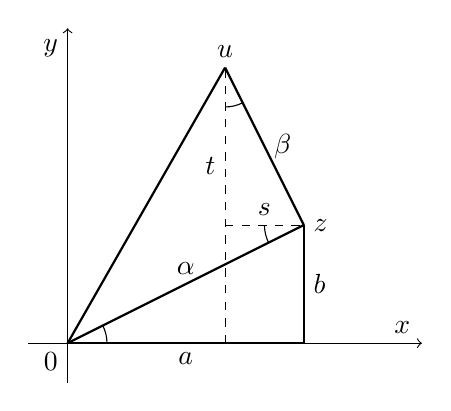
\begin{tikzpicture}[x=0.5cm,y=0.5cm]
    	\draw[->] (-1,0) -- (9,0);
      \draw[->] (0,-1) -- (0,8);
      %
      \draw[thick] (0,0) -- (6,0);
      \draw[thick] (0,0) -- (6,3);
      \draw[thick] (0,0) -- (4,7);
      \draw[thick] (6,0) -- (6,3);
      \draw[thick] (6,3) -- (4,7);
      %
      \draw[dashed] (4,0) -- (4,7);
      \draw[dashed] (4,3) -- (6,3);
      %
      \draw (1,0) arc (0:{atan(1/2)}:1);
      \draw (6,3)+(-1,0) arc (180:{180+atan(1/2)}:1);
      \draw (4,7)+(0,-1) arc (-90:{-90+atan(1/2)}:1);
      %
      \node[below] at (3,0) {$a$};
      \node[right] at (6,1.5) {$b$};
      \node[above] at (3,1.5) {$\alpha$};
      \node[right] at (5,5) {$\beta$};
      \node[above] at (5,3) {$s$};
      \node[left] at (4,4.5) {$t$};
      \node[right] at (6,3) {$z$};
      \node[above] at (4,7) {$u$};
      \node[above] at (8.5,0) {$x$};
      \node[left] at (0,7.5) {$y$};
      \node[below left] at (0,0) {$0$};
    \end{tikzpicture}
  \end{center}
  \caption{Consideriamo i numeri complessi $z=a+ib$ e $w=\alpha+i\beta$
  e supponiamo che sia $\alpha^2 = a^2+b^2$.
  Si consideri il punto $u$ che si ottiene ruotando il punto $w$ dell'angolo
  individuato dal punto $z$. Si avrà allora $u=a-s + i(b+t)$ dove $s$ e $t$
  sono i cateti del triangolo rettangolo con ipotenusa $\beta$.
  Grazie alle proprietà di similitudine dei triangoli si ha
  $\frac{s}{\beta} = \frac{b}{\alpha}$ e $\frac{t}{\beta} = \frac{a}{\alpha}$
  da cui si ottiene quindi $u = a-\frac{b\beta}{\alpha}+i(b+\frac{a\beta}{\alpha})$
  ovvero $\alpha u = (a\alpha - b \beta) + i (b\alpha + a \beta) = z\cdot w$.
  Significa che il numero complesso $z\cdot w$ si trova sulla semiretta
  che individua un angolo che è la somma degli angoli individuati
  dai numeri complessi $z$ e $w$.
  }
  \label{fig:prodotto_complesso}
\end{figure}

Possiamo ora dare una interpretazione geometrica del prodotto $z\cdot w$
tra due numeri complessi. In primo luogo sappiamo che $\abs{z\cdot w} = \abs{z} \cdot \abs{w}$ e dunque il punto del piano che rappresenta il prodotto $z\cdot w$ si trova ad una distanza dall'origine che è pari al prodotto delle distanze
dei punti $z$ e $w$. Inoltre l'angolo individuato da $z\cdot w$ rispetto
all'asse delle $x$ positive risulta uguale alla somma
degli angoli individuati dai punti $z$ e $w$ come mostrato in figura~\ref{fig:prodotto_complesso}.

Anche lo spazio dei numeri complessi può essere esteso aggiungendoci
un punto all'\myemph{infinito}.
A differenza dei reali, su cui era presente un ordinamento che era utile conservare,
nel caso dei numeri complessi è più usuale utilizzare un unico punto infinito
che si denota con \myemph{$\infty$}.
Definiamo lo spazio dei complessi estesi $\bar \CC$ come
\[
\bar \CC = \CC \cup \ENCLOSE{\infty}.
\]
Definiamo
\begin{align*}
  z + \infty &= \infty \qquad \forall z \in \CC\\
  z - \infty &= \infty \qquad \forall z \in \CC\\
   z\cdot \infty &= \infty \qquad \forall z \in \bar\CC\setminus\ENCLOSE{0} \\
   z / \infty &= 0 \qquad \forall z \in \CC \\
   z / 0 &= \infty \qquad \forall z \in \bar \CC \setminus\ENCLOSE{0}\\
   \abs{\infty} &= +\infty \in \bar \RR.
\end{align*}
Si noti che abbiamo definito la divisione per zero di numeri complessi
(e quindi anche reali) diversi da zero. Il risultato è $\infty$ e quindi
rimane confermato che la divisione per zero non è una operazione valida
se vogliamo un risultato finito.
Una quantità $z\in \bar \CC$ sarà detta \emph{finita} se $z\in \CC$.

La definizione di continuità per le funzioni complesse di variabile complessa
è formalmente identica a quella già data per le funzioni reali.
Si tratta semplicemente di sostituire il valore assoluto con il modulo complesso.
%
\begin{definition}[continuità in $\CC$]
Una funzione $f\colon A \subset \CC \to \CC$ è
continua nel punto $z_0\in A$ se
\[
\forall \eps>0\colon \exists \delta>0 \colon \forall z\in A\colon
\abs{z-z_0}<\delta \implies \abs{f(z)-f(z_0)} < \eps.
\]

La funzione $f$ si dice essere \emph{continua} se
è continua in ogni punto $z_0\in A$.
\end{definition}

Anche i teoremi sulla continuità della composizione di funzioni
continue valgono identici e con la stessa dimostrazione
se le funzioni hanno variabile e valori complessi.
Osserviamo che questo vale
in particolare anche per funzioni complesse di variabile reale
$f\colon \RR\to \CC$ e per funzioni reali di variabile complessa
$f\colon \CC \to \RR$.

%%%%%%%%%%%%%%%%%%%
%%%%%%%%%%%%%%%%%%%
%%%%%%%%%%%%%%%%%%%
